%%%%%%%%%%%%%%%%%%%%%%%%%%%%%%%%%%%%%%%%%
% Masters/Doctoral Thesis 
% LaTeX Template
% Version 2.5 (27/8/17)
%
% This template was downloaded from:
% http://www.LaTeXTemplates.com
%
% Version 2.x major modifications by:
% Vel (vel@latextemplates.com)
%
% This template is based on a template by:
% Steve Gunn (http://users.ecs.soton.ac.uk/srg/softwaretools/document/templates/)
% Sunil Patel (http://www.sunilpatel.co.uk/thesis-template/)
%
% Template license:
% CC BY-NC-SA 3.0 (http://creativecommons.org/licenses/by-nc-sa/3.0/)
%
%%%%%%%%%%%%%%%%%%%%%%%%%%%%%%%%%%%%%%%%%

%----------------------------------------------------------------------------------------
%	PACKAGES AND OTHER DOCUMENT CONFIGURATIONS
%----------------------------------------------------------------------------------------

\documentclass[
11pt, % The default document font size, options: 10pt, 11pt, 12pt
%oneside, % Two side (alternating margins) for binding by default, uncomment to switch to one side
english, % ngerman for German
singlespacing, % Single line spacing, alternatives: onehalfspacing or doublespacing
%draft, % Uncomment to enable draft mode (no pictures, no links, overfull hboxes indicated)
%nolistspacing, % If the document is onehalfspacing or doublespacing, uncomment this to set spacing in lists to single
%liststotoc, % Uncomment to add the list of figures/tables/etc to the table of contents
%toctotoc, % Uncomment to add the main table of contents to the table of contents
%parskip, % Uncomment to add space between paragraphs
%nohyperref, % Uncomment to not load the hyperref package
headsepline, % Uncomment to get a line under the header
%chapterinoneline, % Uncomment to place the chapter title next to the number on one line
%consistentlayout, % Uncomment to change the layout of the declaration, abstract and acknowledgements pages to match the default layout
]{MastersDoctoralThesis} % The class file specifying the document structure

\usepackage[utf8]{inputenc} % Required for inputting international characters
\usepackage[T1]{fontenc} % Output font encoding for international characters

\usepackage{mathpazo} % Use the Palatino font by default

\usepackage[backend=bibtex,style=authoryear,natbib=true]{biblatex} % Use the bibtex backend with the authoryear citation style (which resembles APA)

\addbibresource{bibl.bib} % The filename of the bibliography

\usepackage[autostyle=true]{csquotes} % Required to generate language-dependent quotes in the bibliography


%-------------AXEL PACKAGES----------------------
\usepackage{graphicx}
\usepackage{amsmath}

\usepackage{xcolor}
\usepackage{amssymb}
\usepackage{amsmath}
\usepackage{subcaption}
\usepackage{algorithm}
\usepackage{algpseudocode}
\usepackage{hyperref}


\usepackage{rotating}
\usepackage{tikz}
\usepackage{multicol}
\graphicspath{{../figs/}}
\newtheorem{proof}{Proof}
\newtheorem{lemma}{Lemma}

%----------------------------------------------------------------------------------------
%	MARGIN SETTINGS
%----------------------------------------------------------------------------------------

\geometry{
	paper=a4paper, % Change to letterpaper for US letter
	inner=2.5cm, % Inner margin
	outer=2.5cm, % Outer margin
	bindingoffset=.5cm, % Binding offset
	top=1.5cm, % Top margin
	bottom=1.5cm, % Bottom margin
	%showframe, % Uncomment to show how the type block is set on the page
}

%----------------------------------------------------------------------------------------
%	THESIS INFORMATION
%----------------------------------------------------------------------------------------

\thesistitle{Sequential Cognition Processes: A Framework For Reasoning with Non-Monotonic Logics} % Your thesis title, this is used in the title and abstract, print it elsewhere with \ttitle
\supervisor{Dr. Marco \textsc{Ragni}} % Your supervisor's name, this is used in the title page, print it elsewhere with \supname
\examiner{} % Your examiner's name, this is not currently used anywhere in the template, print it elsewhere with \examname
\degree{Master of Computer Science} % Your degree name, this is used in the title page and abstract, print it elsewhere with \degreename
\author{Axel \textsc{Ind}} % Your name, this is used in the title page and abstract, print it elsewhere with \authorname
\addresses{} % Your address, this is not currently used anywhere in the template, print it elsewhere with \addressname

\subject{Computer Science} % Your subject area, this is not currently used anywhere in the template, print it elsewhere with \subjectname
\keywords{} % Keywords for your thesis, this is not currently used anywhere in the template, print it elsewhere with \keywordnames
\university{\href{https://www.uni-freiburg.de}{Albert-Ludwigs-Universit{\"a}t Freiburg}} % Your university's name and URL, this is used in the title page and abstract, print it elsewhere with \univname
\department{\href{http://www.informatik.uni-freiburg.de}{Department of Computer Science}} % Your department's name and URL, this is used in the title page and abstract, print it elsewhere with \deptname
\group{\href{https://www.cognitive-computation.uni-freiburg.de}{Cognitive Computation}} % Your research group's name and URL, this is used in the title page, print it elsewhere with \groupname
\faculty{\href{http://www.tf.uni-freiburg.de}{Faculty of Engineering}} % Your faculty's name and URL, this is used in the title page and abstract, print it elsewhere with \facname

\AtBeginDocument{
\hypersetup{pdftitle=\ttitle} % Set the PDF's title to your title
\hypersetup{pdfauthor=\authorname} % Set the PDF's author to your name
\hypersetup{pdfkeywords=\keywordnames} % Set the PDF's keywords to your keywords
}

\begin{document}

\frontmatter % Use roman page numbering style (i, ii, iii, iv...) for the pre-content pages

\pagestyle{plain} % Default to the plain heading style until the thesis style is called for the body content

%----------------------------------------------------------------------------------------
%	TITLE PAGE
%----------------------------------------------------------------------------------------

\begin{titlepage}
\begin{center}

\vspace*{.06\textheight}
{\scshape\LARGE \univname\par}\vspace{1.5cm} % University name
\textsc{\Large Master's Thesis}\\[0.5cm] % Thesis type

\HRule \\[0.4cm] % Horizontal line
{\huge \bfseries \ttitle\par}\vspace{0.4cm} % Thesis title
\HRule \\[1.5cm] % Horizontal line
 
\begin{minipage}[t]{0.4\textwidth}
\begin{flushleft} \large
\emph{Author:}\\
\href{http://www.johnsmith.com}{\authorname} % Author name - remove the \href bracket to remove the link
\end{flushleft}
\end{minipage}
\begin{minipage}[t]{0.4\textwidth}
\begin{flushright} \large
\emph{Supervisor:} \\
\href{http://www.jamessmith.com}{\supname} % Supervisor name - remove the \href bracket to remove the link  
\end{flushright}
\end{minipage}\\[3cm]
 
\vfill

\large \textit{A thesis submitted in fulfillment of the requirements\\ for the degree of \degreename}\\[0.3cm] % University requirement text
\textit{in the}\\[0.4cm]
\groupname\\\deptname\\[2cm] % Research group name and department name
 
\vfill

{\large \today}\\[4cm] % Date
%\includegraphics{Logo} % University/department logo - uncomment to place it
 
\vfill
\end{center}
\end{titlepage}

%----------------------------------------------------------------------------------------
%	DECLARATION PAGE
%----------------------------------------------------------------------------------------

\begin{declaration}
\addchaptertocentry{\authorshipname} % Add the declaration to the table of contents
\noindent I, \authorname, declare that this thesis titled, \enquote{\ttitle} and the work presented in it are my own. I confirm that:

\begin{itemize} 
\item This work was done wholly or mainly while in candidature for a research degree at this University.
\item Where any part of this thesis has previously been submitted for a degree or any other qualification at this University or any other institution, this has been clearly stated.
\item Where I have consulted the published work of others, this is always clearly attributed.
\item Where I have quoted from the work of others, the source is always given. With the exception of such quotations, this thesis is entirely my own work.
\item I have acknowledged all main sources of help.
\item Where the thesis is based on work done by myself jointly with others, I have made clear exactly what was done by others and what I have contributed myself.\\
\end{itemize}
 
\noindent Signed:\\
\rule[0.5em]{25em}{0.5pt} % This prints a line for the signature
 
\noindent Date:\\
\rule[0.5em]{25em}{0.5pt} % This prints a line to write the date
\end{declaration}

\cleardoublepage

%----------------------------------------------------------------------------------------
%	QUOTATION PAGE
%----------------------------------------------------------------------------------------

\vspace*{0.2\textheight}

\noindent\enquote{\itshape Everything should be made as simple as possible, but no simpler.}\bigbreak

\hfill Albert Einstein

%----------------------------------------------------------------------------------------
%	ABSTRACT PAGE
%----------------------------------------------------------------------------------------

\begin{abstract}
\addchaptertocentry{\abstractname} % Add the abstract to the table of contents
Approaches to cognitive modelling with non-monotonic logics have thus far been largely \textit{ad hoc} and poorly standardised, making inter-model comparisons difficult. As an attempt to systematically represent non-monotonic logics in a framework that standardises cognitive modelling under these logics without sacrificing their expressiveness, we introduce the Sequential Cognition Process (SCP). Under the assumption that human reasoning can be represented as a sequence of distinct cognitive operations on an initial knowledge base SCPs provide a consistent framework for generating and evaluating models of human cognition. Using an adapted interpretation of the Weak Completion Semantics (WCS), SCPs are able to accurately model several classical experiments in cognitive modelling. We use the SCP framework to model both general case reasoners -- which arrive at the most frequently observed conclusions -- and poorly-studied individual case reasoners -- which do not. We illustrate the use of SCPs using the Suppression Task.
\end{abstract}

%----------------------------------------------------------------------------------------
%	ACKNOWLEDGEMENTS
%----------------------------------------------------------------------------------------

\begin{acknowledgements}
\addchaptertocentry{\acknowledgementname} % Add the acknowledgements to the table of contents
Special thanks to Dr. Marco Ragni, for his enthusiastic supervision of my ongoing academic studies; Raymond Ind and Julie Ind for their emotional and financial support; and to Anastasia Sushich for her tireless support.
\end{acknowledgements}

%----------------------------------------------------------------------------------------
%	LIST OF CONTENTS/FIGURES/TABLES PAGES
%----------------------------------------------------------------------------------------

\tableofcontents % Prints the main table of contents

\listoffigures % Prints the list of figures

\listoftables % Prints the list of tables

%----------------------------------------------------------------------------------------
%	ABBREVIATIONS
%----------------------------------------------------------------------------------------

\begin{abbreviations}{ll} % Include a list of abbreviations (a table of two columns)

\textbf{SCP} & \textbf{S}equential \textbf{C}ognitive \textbf{P}rocesses\\
\textbf{WCS} & \textbf{W}eak \textbf{C}ompletion \textbf{S}emantics\\
\textbf{WST} & \textbf{W}ason \textbf{S}election \textbf{T}ask

\end{abbreviations}

%----------------------------------------------------------------------------------------
%	THESIS CONTENT - CHAPTERS
%----------------------------------------------------------------------------------------

\mainmatter % Begin numeric (1,2,3...) page numbering

\pagestyle{thesis} % Return the page headers back to the "thesis" style

% Include the chapters of the thesis as separate files from the Chapters folder
% Uncomment the lines as you write the chapters
@TODO include chapters as shown below
%% Chapter 1

\chapter{Chapter Title Here} % Main chapter title

\label{Chapter1} % For referencing the chapter elsewhere, use \ref{Chapter1} 

%----------------------------------------------------------------------------------------

% Define some commands to keep the formatting separated from the content 
\newcommand{\keyword}[1]{\textbf{#1}}
\newcommand{\tabhead}[1]{\textbf{#1}}
\newcommand{\code}[1]{\texttt{#1}}
\newcommand{\file}[1]{\texttt{\bfseries#1}}
\newcommand{\option}[1]{\texttt{\itshape#1}}

%----------------------------------------------------------------------------------------

\section{Welcome and Thank You}
Welcome to this \LaTeX{} Thesis Template, a beautiful and easy to use template for writing a thesis using the \LaTeX{} typesetting system.

If you are writing a thesis (or will be in the future) and its subject is technical or mathematical (though it doesn't have to be), then creating it in \LaTeX{} is highly recommended as a way to make sure you can just get down to the essential writing without having to worry over formatting or wasting time arguing with your word processor.

\LaTeX{} is easily able to professionally typeset documents that run to hundreds or thousands of pages long. With simple mark-up commands, it automatically sets out the table of contents, margins, page headers and footers and keeps the formatting consistent and beautiful. One of its main strengths is the way it can easily typeset mathematics, even \emph{heavy} mathematics. Even if those equations are the most horribly twisted and most difficult mathematical problems that can only be solved on a super-computer, you can at least count on \LaTeX{} to make them look stunning.

%----------------------------------------------------------------------------------------

\section{Learning \LaTeX{}}

\LaTeX{} is not a \textsc{wysiwyg} (What You See is What You Get) program, unlike word processors such as Microsoft Word or Apple's Pages. Instead, a document written for \LaTeX{} is actually a simple, plain text file that contains \emph{no formatting}. You tell \LaTeX{} how you want the formatting in the finished document by writing in simple commands amongst the text, for example, if I want to use \emph{italic text for emphasis}, I write the \verb|\emph{text}| command and put the text I want in italics in between the curly braces. This means that \LaTeX{} is a \enquote{mark-up} language, very much like HTML.

\subsection{A (not so short) Introduction to \LaTeX{}}

If you are new to \LaTeX{}, there is a very good eBook -- freely available online as a PDF file -- called, \enquote{The Not So Short Introduction to \LaTeX{}}. The book's title is typically shortened to just \emph{lshort}. You can download the latest version (as it is occasionally updated) from here:
\url{http://www.ctan.org/tex-archive/info/lshort/english/lshort.pdf}

It is also available in several other languages. Find yours from the list on this page: \url{http://www.ctan.org/tex-archive/info/lshort/}

It is recommended to take a little time out to learn how to use \LaTeX{} by creating several, small `test' documents, or having a close look at several templates on:\\ 
\url{http://www.LaTeXTemplates.com}\\ 
Making the effort now means you're not stuck learning the system when what you \emph{really} need to be doing is writing your thesis.

\subsection{A Short Math Guide for \LaTeX{}}

If you are writing a technical or mathematical thesis, then you may want to read the document by the AMS (American Mathematical Society) called, \enquote{A Short Math Guide for \LaTeX{}}. It can be found online here:
\url{http://www.ams.org/tex/amslatex.html}
under the \enquote{Additional Documentation} section towards the bottom of the page.

\subsection{Common \LaTeX{} Math Symbols}
There are a multitude of mathematical symbols available for \LaTeX{} and it would take a great effort to learn the commands for them all. The most common ones you are likely to use are shown on this page:
\url{http://www.sunilpatel.co.uk/latex-type/latex-math-symbols/}

You can use this page as a reference or crib sheet, the symbols are rendered as large, high quality images so you can quickly find the \LaTeX{} command for the symbol you need.

\subsection{\LaTeX{} on a Mac}
 
The \LaTeX{} distribution is available for many systems including Windows, Linux and Mac OS X. The package for OS X is called MacTeX and it contains all the applications you need -- bundled together and pre-customized -- for a fully working \LaTeX{} environment and work flow.
 
MacTeX includes a custom dedicated \LaTeX{} editor called TeXShop for writing your `\file{.tex}' files and BibDesk: a program to manage your references and create your bibliography section just as easily as managing songs and creating playlists in iTunes.

%----------------------------------------------------------------------------------------

\section{Getting Started with this Template}

If you are familiar with \LaTeX{}, then you should explore the directory structure of the template and then proceed to place your own information into the \emph{THESIS INFORMATION} block of the \file{main.tex} file. You can then modify the rest of this file to your unique specifications based on your degree/university. Section \ref{FillingFile} on page \pageref{FillingFile} will help you do this. Make sure you also read section \ref{ThesisConventions} about thesis conventions to get the most out of this template.

If you are new to \LaTeX{} it is recommended that you carry on reading through the rest of the information in this document.

Before you begin using this template you should ensure that its style complies with the thesis style guidelines imposed by your institution. In most cases this template style and layout will be suitable. If it is not, it may only require a small change to bring the template in line with your institution's recommendations. These modifications will need to be done on the \file{MastersDoctoralThesis.cls} file.

\subsection{About this Template}

This \LaTeX{} Thesis Template is originally based and created around a \LaTeX{} style file created by Steve R.\ Gunn from the University of Southampton (UK), department of Electronics and Computer Science. You can find his original thesis style file at his site, here:
\url{http://www.ecs.soton.ac.uk/~srg/softwaretools/document/templates/}

Steve's \file{ecsthesis.cls} was then taken by Sunil Patel who modified it by creating a skeleton framework and folder structure to place the thesis files in. The resulting template can be found on Sunil's site here:
\url{http://www.sunilpatel.co.uk/thesis-template}

Sunil's template was made available through \url{http://www.LaTeXTemplates.com} where it was modified many times based on user requests and questions. Version 2.0 and onwards of this template represents a major modification to Sunil's template and is, in fact, hardly recognisable. The work to make version 2.0 possible was carried out by \href{mailto:vel@latextemplates.com}{Vel} and Johannes Böttcher.

%----------------------------------------------------------------------------------------

\section{What this Template Includes}

\subsection{Folders}

This template comes as a single zip file that expands out to several files and folders. The folder names are mostly self-explanatory:

\keyword{Appendices} -- this is the folder where you put the appendices. Each appendix should go into its own separate \file{.tex} file. An example and template are included in the directory.

\keyword{Chapters} -- this is the folder where you put the thesis chapters. A thesis usually has about six chapters, though there is no hard rule on this. Each chapter should go in its own separate \file{.tex} file and they can be split as:
\begin{itemize}
\item Chapter 1: Introduction to the thesis topic
\item Chapter 2: Background information and theory
\item Chapter 3: (Laboratory) experimental setup
\item Chapter 4: Details of experiment 1
\item Chapter 5: Details of experiment 2
\item Chapter 6: Discussion of the experimental results
\item Chapter 7: Conclusion and future directions
\end{itemize}
This chapter layout is specialised for the experimental sciences, your discipline may be different.

\keyword{Figures} -- this folder contains all figures for the thesis. These are the final images that will go into the thesis document.

\subsection{Files}

Included are also several files, most of them are plain text and you can see their contents in a text editor. After initial compilation, you will see that more auxiliary files are created by \LaTeX{} or BibTeX and which you don't need to delete or worry about:

\keyword{example.bib} -- this is an important file that contains all the bibliographic information and references that you will be citing in the thesis for use with BibTeX. You can write it manually, but there are reference manager programs available that will create and manage it for you. Bibliographies in \LaTeX{} are a large subject and you may need to read about BibTeX before starting with this. Many modern reference managers will allow you to export your references in BibTeX format which greatly eases the amount of work you have to do.

\keyword{MastersDoctoralThesis.cls} -- this is an important file. It is the class file that tells \LaTeX{} how to format the thesis. 

\keyword{main.pdf} -- this is your beautifully typeset thesis (in the PDF file format) created by \LaTeX{}. It is supplied in the PDF with the template and after you compile the template you should get an identical version.

\keyword{main.tex} -- this is an important file. This is the file that you tell \LaTeX{} to compile to produce your thesis as a PDF file. It contains the framework and constructs that tell \LaTeX{} how to layout the thesis. It is heavily commented so you can read exactly what each line of code does and why it is there. After you put your own information into the \emph{THESIS INFORMATION} block -- you have now started your thesis!

Files that are \emph{not} included, but are created by \LaTeX{} as auxiliary files include:

\keyword{main.aux} -- this is an auxiliary file generated by \LaTeX{}, if it is deleted \LaTeX{} simply regenerates it when you run the main \file{.tex} file.

\keyword{main.bbl} -- this is an auxiliary file generated by BibTeX, if it is deleted, BibTeX simply regenerates it when you run the \file{main.aux} file. Whereas the \file{.bib} file contains all the references you have, this \file{.bbl} file contains the references you have actually cited in the thesis and is used to build the bibliography section of the thesis.

\keyword{main.blg} -- this is an auxiliary file generated by BibTeX, if it is deleted BibTeX simply regenerates it when you run the main \file{.aux} file.

\keyword{main.lof} -- this is an auxiliary file generated by \LaTeX{}, if it is deleted \LaTeX{} simply regenerates it when you run the main \file{.tex} file. It tells \LaTeX{} how to build the \emph{List of Figures} section.

\keyword{main.log} -- this is an auxiliary file generated by \LaTeX{}, if it is deleted \LaTeX{} simply regenerates it when you run the main \file{.tex} file. It contains messages from \LaTeX{}, if you receive errors and warnings from \LaTeX{}, they will be in this \file{.log} file.

\keyword{main.lot} -- this is an auxiliary file generated by \LaTeX{}, if it is deleted \LaTeX{} simply regenerates it when you run the main \file{.tex} file. It tells \LaTeX{} how to build the \emph{List of Tables} section.

\keyword{main.out} -- this is an auxiliary file generated by \LaTeX{}, if it is deleted \LaTeX{} simply regenerates it when you run the main \file{.tex} file.

So from this long list, only the files with the \file{.bib}, \file{.cls} and \file{.tex} extensions are the most important ones. The other auxiliary files can be ignored or deleted as \LaTeX{} and BibTeX will regenerate them.

%----------------------------------------------------------------------------------------

\section{Filling in Your Information in the \file{main.tex} File}\label{FillingFile}

You will need to personalise the thesis template and make it your own by filling in your own information. This is done by editing the \file{main.tex} file in a text editor or your favourite LaTeX environment.

Open the file and scroll down to the third large block titled \emph{THESIS INFORMATION} where you can see the entries for \emph{University Name}, \emph{Department Name}, etc \ldots

Fill out the information about yourself, your group and institution. You can also insert web links, if you do, make sure you use the full URL, including the \code{http://} for this. If you don't want these to be linked, simply remove the \verb|\href{url}{name}| and only leave the name.

When you have done this, save the file and recompile \code{main.tex}. All the information you filled in should now be in the PDF, complete with web links. You can now begin your thesis proper!

%----------------------------------------------------------------------------------------

\section{The \code{main.tex} File Explained}

The \file{main.tex} file contains the structure of the thesis. There are plenty of written comments that explain what pages, sections and formatting the \LaTeX{} code is creating. Each major document element is divided into commented blocks with titles in all capitals to make it obvious what the following bit of code is doing. Initially there seems to be a lot of \LaTeX{} code, but this is all formatting, and it has all been taken care of so you don't have to do it.

Begin by checking that your information on the title page is correct. For the thesis declaration, your institution may insist on something different than the text given. If this is the case, just replace what you see with what is required in the \emph{DECLARATION PAGE} block.

Then comes a page which contains a funny quote. You can put your own, or quote your favourite scientist, author, person, and so on. Make sure to put the name of the person who you took the quote from.

Following this is the abstract page which summarises your work in a condensed way and can almost be used as a standalone document to describe what you have done. The text you write will cause the heading to move up so don't worry about running out of space.

Next come the acknowledgements. On this page, write about all the people who you wish to thank (not forgetting parents, partners and your advisor/supervisor).

The contents pages, list of figures and tables are all taken care of for you and do not need to be manually created or edited. The next set of pages are more likely to be optional and can be deleted since they are for a more technical thesis: insert a list of abbreviations you have used in the thesis, then a list of the physical constants and numbers you refer to and finally, a list of mathematical symbols used in any formulae. Making the effort to fill these tables means the reader has a one-stop place to refer to instead of searching the internet and references to try and find out what you meant by certain abbreviations or symbols.

The list of symbols is split into the Roman and Greek alphabets. Whereas the abbreviations and symbols ought to be listed in alphabetical order (and this is \emph{not} done automatically for you) the list of physical constants should be grouped into similar themes.

The next page contains a one line dedication. Who will you dedicate your thesis to?

Finally, there is the block where the chapters are included. Uncomment the lines (delete the \code{\%} character) as you write the chapters. Each chapter should be written in its own file and put into the \emph{Chapters} folder and named \file{Chapter1}, \file{Chapter2}, etc\ldots Similarly for the appendices, uncomment the lines as you need them. Each appendix should go into its own file and placed in the \emph{Appendices} folder.

After the preamble, chapters and appendices finally comes the bibliography. The bibliography style (called \option{authoryear}) is used for the bibliography and is a fully featured style that will even include links to where the referenced paper can be found online. Do not underestimate how grateful your reader will be to find that a reference to a paper is just a click away. Of course, this relies on you putting the URL information into the BibTeX file in the first place.

%----------------------------------------------------------------------------------------

\section{Thesis Features and Conventions}\label{ThesisConventions}

To get the best out of this template, there are a few conventions that you may want to follow.

One of the most important (and most difficult) things to keep track of in such a long document as a thesis is consistency. Using certain conventions and ways of doing things (such as using a Todo list) makes the job easier. Of course, all of these are optional and you can adopt your own method.

\subsection{Printing Format}

This thesis template is designed for double sided printing (i.e. content on the front and back of pages) as most theses are printed and bound this way. Switching to one sided printing is as simple as uncommenting the \option{oneside} option of the \code{documentclass} command at the top of the \file{main.tex} file. You may then wish to adjust the margins to suit specifications from your institution.

The headers for the pages contain the page number on the outer side (so it is easy to flick through to the page you want) and the chapter name on the inner side.

The text is set to 11 point by default with single line spacing, again, you can tune the text size and spacing should you want or need to using the options at the very start of \file{main.tex}. The spacing can be changed similarly by replacing the \option{singlespacing} with \option{onehalfspacing} or \option{doublespacing}.

\subsection{Using US Letter Paper}

The paper size used in the template is A4, which is the standard size in Europe. If you are using this thesis template elsewhere and particularly in the United States, then you may have to change the A4 paper size to the US Letter size. This can be done in the margins settings section in \file{main.tex}.

Due to the differences in the paper size, the resulting margins may be different to what you like or require (as it is common for institutions to dictate certain margin sizes). If this is the case, then the margin sizes can be tweaked by modifying the values in the same block as where you set the paper size. Now your document should be set up for US Letter paper size with suitable margins.

\subsection{References}

The \code{biblatex} package is used to format the bibliography and inserts references such as this one \parencite{Reference1}. The options used in the \file{main.tex} file mean that the in-text citations of references are formatted with the author(s) listed with the date of the publication. Multiple references are separated by semicolons (e.g. \parencite{Reference2, Reference1}) and references with more than three authors only show the first author with \emph{et al.} indicating there are more authors (e.g. \parencite{Reference3}). This is done automatically for you. To see how you use references, have a look at the \file{Chapter1.tex} source file. Many reference managers allow you to simply drag the reference into the document as you type.

Scientific references should come \emph{before} the punctuation mark if there is one (such as a comma or period). The same goes for footnotes\footnote{Such as this footnote, here down at the bottom of the page.}. You can change this but the most important thing is to keep the convention consistent throughout the thesis. Footnotes themselves should be full, descriptive sentences (beginning with a capital letter and ending with a full stop). The APA6 states: \enquote{Footnote numbers should be superscripted, [...], following any punctuation mark except a dash.} The Chicago manual of style states: \enquote{A note number should be placed at the end of a sentence or clause. The number follows any punctuation mark except the dash, which it precedes. It follows a closing parenthesis.}

The bibliography is typeset with references listed in alphabetical order by the first author's last name. This is similar to the APA referencing style. To see how \LaTeX{} typesets the bibliography, have a look at the very end of this document (or just click on the reference number links in in-text citations).

\subsubsection{A Note on bibtex}

The bibtex backend used in the template by default does not correctly handle unicode character encoding (i.e. "international" characters). You may see a warning about this in the compilation log and, if your references contain unicode characters, they may not show up correctly or at all. The solution to this is to use the biber backend instead of the outdated bibtex backend. This is done by finding this in \file{main.tex}: \option{backend=bibtex} and changing it to \option{backend=biber}. You will then need to delete all auxiliary BibTeX files and navigate to the template directory in your terminal (command prompt). Once there, simply type \code{biber main} and biber will compile your bibliography. You can then compile \file{main.tex} as normal and your bibliography will be updated. An alternative is to set up your LaTeX editor to compile with biber instead of bibtex, see \href{http://tex.stackexchange.com/questions/154751/biblatex-with-biber-configuring-my-editor-to-avoid-undefined-citations/}{here} for how to do this for various editors.

\subsection{Tables}

Tables are an important way of displaying your results, below is an example table which was generated with this code:

{\small
\begin{verbatim}
\begin{table}
\caption{The effects of treatments X and Y on the four groups studied.}
\label{tab:treatments}
\centering
\begin{tabular}{l l l}
\toprule
\tabhead{Groups} & \tabhead{Treatment X} & \tabhead{Treatment Y} \\
\midrule
1 & 0.2 & 0.8\\
2 & 0.17 & 0.7\\
3 & 0.24 & 0.75\\
4 & 0.68 & 0.3\\
\bottomrule\\
\end{tabular}
\end{table}
\end{verbatim}
}

\begin{table}
\caption{The effects of treatments X and Y on the four groups studied.}
\label{tab:treatments}
\centering
\begin{tabular}{l l l}
\toprule
\tabhead{Groups} & \tabhead{Treatment X} & \tabhead{Treatment Y} \\
\midrule
1 & 0.2 & 0.8\\
2 & 0.17 & 0.7\\
3 & 0.24 & 0.75\\
4 & 0.68 & 0.3\\
\bottomrule\\
\end{tabular}
\end{table}

You can reference tables with \verb|\ref{<label>}| where the label is defined within the table environment. See \file{Chapter1.tex} for an example of the label and citation (e.g. Table~\ref{tab:treatments}).

\subsection{Figures}

There will hopefully be many figures in your thesis (that should be placed in the \emph{Figures} folder). The way to insert figures into your thesis is to use a code template like this:
\begin{verbatim}
\begin{figure}
\centering

\includegraphics{Figures/Electron}
\decoRule
\caption[An Electron]{An electron (artist's impression).}
\label{fig:Electron}
\end{figure}
\end{verbatim}
Also look in the source file. Putting this code into the source file produces the picture of the electron that you can see in the figure below.

\begin{figure}[th]
\centering

\includegraphics{Figures/Electron}
\decoRule
\caption[An Electron]{An electron (artist's impression).}
\label{fig:Electron}
\end{figure}

Sometimes figures don't always appear where you write them in the source. The placement depends on how much space there is on the page for the figure. Sometimes there is not enough room to fit a figure directly where it should go (in relation to the text) and so \LaTeX{} puts it at the top of the next page. Positioning figures is the job of \LaTeX{} and so you should only worry about making them look good!

Figures usually should have captions just in case you need to refer to them (such as in Figure~\ref{fig:Electron}). The \verb|\caption| command contains two parts, the first part, inside the square brackets is the title that will appear in the \emph{List of Figures}, and so should be short. The second part in the curly brackets should contain the longer and more descriptive caption text.

The \verb|\decoRule| command is optional and simply puts an aesthetic horizontal line below the image. If you do this for one image, do it for all of them.

\LaTeX{} is capable of using images in pdf, jpg and png format.

\subsection{Typesetting mathematics}

If your thesis is going to contain heavy mathematical content, be sure that \LaTeX{} will make it look beautiful, even though it won't be able to solve the equations for you.

The \enquote{Not So Short Introduction to \LaTeX} (available on \href{http://www.ctan.org/tex-archive/info/lshort/english/lshort.pdf}{CTAN}) should tell you everything you need to know for most cases of typesetting mathematics. If you need more information, a much more thorough mathematical guide is available from the AMS called, \enquote{A Short Math Guide to \LaTeX} and can be downloaded from:
\url{ftp://ftp.ams.org/pub/tex/doc/amsmath/short-math-guide.pdf}

There are many different \LaTeX{} symbols to remember, luckily you can find the most common symbols in \href{http://ctan.org/pkg/comprehensive}{The Comprehensive \LaTeX~Symbol List}.

You can write an equation, which is automatically given an equation number by \LaTeX{} like this:
\begin{verbatim}
\begin{equation}
E = mc^{2}
\label{eqn:Einstein}
\end{equation}
\end{verbatim}

This will produce Einstein's famous energy-matter equivalence equation:
\begin{equation}
E = mc^{2}
\label{eqn:Einstein}
\end{equation}

All equations you write (which are not in the middle of paragraph text) are automatically given equation numbers by \LaTeX{}. If you don't want a particular equation numbered, use the unnumbered form:
\begin{verbatim}
\[ a^{2}=4 \]
\end{verbatim}

%----------------------------------------------------------------------------------------

\section{Sectioning and Subsectioning}

You should break your thesis up into nice, bite-sized sections and subsections. \LaTeX{} automatically builds a table of Contents by looking at all the \verb|\chapter{}|, \verb|\section{}|  and \verb|\subsection{}| commands you write in the source.

The Table of Contents should only list the sections to three (3) levels. A \verb|chapter{}| is level zero (0). A \verb|\section{}| is level one (1) and so a \verb|\subsection{}| is level two (2). In your thesis it is likely that you will even use a \verb|subsubsection{}|, which is level three (3). The depth to which the Table of Contents is formatted is set within \file{MastersDoctoralThesis.cls}. If you need this changed, you can do it in \file{main.tex}.

%----------------------------------------------------------------------------------------

\section{In Closing}

You have reached the end of this mini-guide. You can now rename or overwrite this pdf file and begin writing your own \file{Chapter1.tex} and the rest of your thesis. The easy work of setting up the structure and framework has been taken care of for you. It's now your job to fill it out!

Good luck and have lots of fun!

\begin{flushright}
Guide written by ---\\
Sunil Patel: \href{http://www.sunilpatel.co.uk}{www.sunilpatel.co.uk}\\
Vel: \href{http://www.LaTeXTemplates.com}{LaTeXTemplates.com}
\end{flushright}

%\include{Chapters/Chapter2} 
%\include{Chapters/Chapter3}
%\include{Chapters/Chapter4} 
%\include{Chapters/Chapter5} 

\chapter{Introduction} \label{chp:intro}
\section{Overview} \label{sec:overview}
% a statement of the problem
The human mind is complex. So complex that thousands of approaches from dozens of fields have failed to capture its complexity. The sheer size of the brain -- containing  over 5000 times as many neurons as the largest practical neural networks \citep{mocanu2018scalable} -- and our limited understanding of the fundamental learning processes it employs mean that researchers can neither completely describe nor predict human actions nor model human thought processes. Instead, much of the current state of the art in cognitive modelling relies on one of two general approaches: creating systems that structurally approximate the human brain, and creating systems which approximate a more abstract intuition of cognition. The first type of system encompasses many algorithms related to machine learning and deep learning; the second type, with which this paper is concerned, has existed in some form for far longer than humans have been thinking creatures \citep{smirnova2015crows}. Every shark stalking its prey, every tiny proto-mammal hiding from a hungry dinosaur, and every man driving to work in the morning, has applied this type of reasoning when trying to make predictions about the actions of other agents in their world. By applying case-specific reasoning to a known world state we are able to make imperfect, but quick, predictions about the mental state of other agents in our world.

Due in part to the difficulty of cloning dinosaurs to hunt participants in cognitive research experiments, and partly due to concerns about the ease with which they could answer questionnaires on the experience later, most cognitive tasks used by researchers tend to be more dull than the examples above.

Non-monotonic logics have proven able to adequately model a large number of standard cognitive reasoning tasks such as The Wason Selection Task\citep{wason1968reasoning} and Suppression Task \citep{byrne1989suppressing}. These approaches, though effective and well-founded in isolation, are often unable to integrate or be compared to data models of other tasks, even when they rely on the same underlying logic. Although the non-monotonic logics themselves are generally carefully described, procedures ranging from best practise in deciding appropriate knowledge bases to the mechanisms by which abnormalities should be created tend to be re-imagined on a case-by-case basis.

Further, cognitive frameworks using non-monotonic logics are almost always designed to describe the most common (general) conclusion drawn by participants in the experiment. Modelling other individual reasoners or classes of reasoners who differ from the norm is often a non-trivial process. It has been shown that the Weak Completion Semantics \citep{holldobler2015weak} is able model the four most general cases of the Wason Selection Task under the assumption that reasoners who differ from the general case (\textit{deviant reasoners}) follow a sequence of mental processes that is still highly similar to that of the general reasoner \citep{breu2019weak}.

This paper introduces the Sequential Cognition Process (SCP) which generalises the assumption of sequential cognitive operations, each of which uses a collection of epistemic states as input and produces a collection of epistemic states as output. Using SCPs and a set of well-founded cognitive operations it is possible to apply traditional search techniques to problems in cognitive modelling with non-monotonic logics that have previously required expert-made models. The SCPs introduce a number of desirable properties: they introduce a partially standardised (though extensible) set of allowable cognitive operations, they standardise the structure of what constitutes an epistemic state, they are easily modified to accommodate deviant reasoners when a well-founded general model already exists, and their sequential structure makes them well-suited to scoring algorithms that allow intra- and inter-experimental modelling and comparisons.


\section{A Review of Terminology} \label{sec:terminology}
% a review of terms
\section{Current State of the Art} \label{sec:soa}
% review of literature
\section{Contributions of the SCP Framework} \label{sec:contributions}
\section{Thesis Layout} \label{sec:layout}
% description of remaining chapters

\chapter{Mathematical Preliminaries}
\subsection{Propositional Logic}

\begin{table}
\begin{center}


\begin{tabular}{ c | c c }
  $\land$& $\top$ & $\bot$ \\ \hline
 $\top$ & $\top$ & $\bot$ \\  
 $\bot$ & $\bot$ &  $\bot$
\end{tabular}
\quad
\begin{tabular}{ c | c c }
  $\lor$& $\top$ & $\bot$ \\ \hline
 $\top$ & $\top$ & $\top$ \\  
 $\bot$ & $\top$ &  $\bot$
\end{tabular}
\quad
\begin{tabular}{ c | c }
  $\lnot$& \\ \hline
 $\top$ & $\bot$ \\  
 $\bot$ & $\top$
\end{tabular}

\begin{tabular}{ c | c c }
  $\rightarrow$& $\top$ & $\bot$ \\ \hline
 $\top$ & $\top$ & $\bot$ \\  
 $\bot$ & $\top$ &  $\top$
\end{tabular}
\quad
\begin{tabular}{ c | c c }
  $\rightarrow$& $\top$ & $\bot$ \\ \hline
 $\top$ & $\top$ & $\bot$ \\  
 $\bot$ & $\bot$ &  $\top$
\end{tabular}

\caption{Truth tables for standard operators in propositional logic.}
\label{tbl:prop}

\end{center}
\end{table}

Propositional (or classical) logic is the form of logic most traditionally associated with problem solving in mathematics and computer science. In propositional logic features of a hypothetical world are encoded by a set of \textit{variables}. every variable must be mapped to either $\top$ (usually denoting truth, in some subject-specific sense) or $\bot$ (denoting falseness). A \textit{clause} $\phi$ consists of either a single atomic variable or an operator and some set of sub-clauses. Every clause has a truth value determined by the values of the sub-clauses it contains and the relevant operator which handles their interaction. Table~\ref{tbl:prop} illustrates the classical interpretations of the allowable operators. A knowledge base $KB$ consists of a set of clauses. In this paper we adopt the assumption all clauses (also called rules) $\in KB$ are of the form $head\leftarrow body$ and all heads are atomic variables.

\section{Logic Programming}

\section{Non-Monotonic Logics}
In the field of non-monotonic logics, reasoning is represented as a collection of defeasible inferences. Unlike in classical logic, conclusions need not hold in perpetuity, or even in the same model and revision is always possible. Monotonic logics are not capable of describing human reasoning in experiments like the Suppression Task \citep{dietz2012computational} because they lack this revisionist characteristic.

A large number of non-monotonic frameworks exist in the literature \citep{mcdermott1980non}, each applicable to a different subset of cognitive problem space, and each modelling their problem space with various degrees of success. In the simplest formulation, a non-monotonic logic is simply an extension to a classical logic which introduces a preference relation $\rightarrow_p$. This preference relation states that, given some number of derivable facts in a knowledge base, the fact derived using the most preferential rule is to be derived first and cannot be overwritten by a less preferable assignment.  

Although the non-monotonic logics discussed in this section has simple extensions to first-order logic, we instead restrict ourselves to a propositional format throughout this thesis.
\section{The Weak Completion Semantics}
\begin{table}
\begin{center}
\begin{tabular}{ c | c c c }
  $\rightarrow$& $\top$ & $u$ & $\bot$ \\ \hline
 $\top$ & $\top$ & $u$ & $\bot$ \\  
 $u$ & $\top$ & $\top$ & $u$\\  
 $\bot$ & $\top$ & $\top$ & $\top$
\end{tabular}
\caption{A table showing the implication operator in 3-valued \L ukasiewicz logic.}
\label{tbl:luk}
\end{center}
\end{table}

The Weak Completion Semantics is a non-monotonic logic which procedurally encodes several well-known cognitive phenomena. The WCS makes use of 3-valued \L ukasiewicz logic (Table~\ref{tbl:luk}). It adds abnormalities to non-ground inferences, and replaces the classical inference ($\leftarrow$), with a bijective ($\leftrightarrow$). 

The Weak Completion of a program $P$ is defined as follows:

\begin{enumerate}
\item Replace all clauses of the form $A \leftarrow body_1$, ..., $A \leftarrow body_n$ with $A \leftarrow body_1 \lor ... \lor body_n$.
% \item For all undefined variables $x$, add $x \leftarrow \bot$. THIS IS FOR STRONG COMPLETION ONLY
\item Replace all occurrences of $\leftarrow$ with $\leftrightarrow$.
\end{enumerate}

Applying this procedure to $P$ results in $wcP$ which is the weak completion of $P$.

The next requirement to apply the WCS framework is the introduction of a semantic operator $\phi_{SvL}$ \citep{stenning2008interpretation}. Let $J$ be the result of applying the semantics operator to an interpretation $I$ and logic program $P$. Then $J$ is defined as follows:

\[
\begin{split}
J^\top = \{ & A | \textrm{ there exists a clause } A\leftarrow Body \in P \\ & \textrm{ with } I(Body) = \top\}
\end{split}
\]
\[
\begin{split}
J^\bot = \{ &  A | \textrm{ there exists a clause } A \leftarrow Body \in P \\
           & \textrm{ and for all clauses } A \leftarrow Body \in P \\ & \textrm{ we find } I(Body) = \bot\}
\end{split}
\]

%this might not be right? Should it say I or J? @TODO
Using $I=<\emptyset, \emptyset>$, the least model of $P$ ($\textrm{lm}_\textrm{\L}$wc$P$) can be calculated by iterating $\phi_{SvL,P}$.

\section{Reiter's Default Logic}
Reteir's Default Logic \citep{reiter1980logic} is a non-monotonic framework which allows us to divide the inferential capabilities of a system into those facts and inference rules which are always true (as in classical logic) and those which are are usually true. The second type of inference is the eponymous default rule.

The set of immutable facts is called $kb$ and inferences in $kb$ are made as with propositional logic, with the addition of the conclusion of any previously evaluated default rules. The set of default rules $d$ consists rules of the form:

\[\frac{\textrm{prerequisite}:\textrm{ justification}_1, \textrm{ ...}, \textrm{ justification}_n}{\textrm{conclusion}}\] @TODOextend.

Where \textit{prerequisite}, $\textit{justification}_i$, and \textit{conclusion} are propositional logic clauses. A \textit{conclusion} is valid and added to the set of known variables in $kb$ iff \textit{prerequisite} holds and no clause $\textit{justification}_i$ holds.

Formally, inferences in default logic are calculated as follows:

@TODOref

It should be immediately apparent form this formulation that, for many possible sets of rules in $kb$, the output is non-monotonic as is dependent on the order in which default rules are evaluated.

A very significant restriction on reiter's default logic is the complexity of computing inferences. Even in the simple case of $kb={rule_1,...rule_n}$ and $d={}$, the set of possible inferences is \textit{NP-complete} as for a propositional formula @TODOnpcompleteref. When default rules are included in this computation the complexity of calculating all possible inferences for all possible default rule application sequences quickly becomes intractable for all but the most basic logic programs. With this limitation in mind, we restrict propositional rules to those in the form $a\leftarrow\phi$ where $a$ is an atomic head. Further, we restrict the set of default rules to those of the form $\frac{B:C}{a}$ where $a$ is an atom.


\chapter{Experiments} \label{chp:experiments}
\section{Suppression Task} \label{sec:sup}
\subsection{Intuitive Overview} \label{ssec:sup_intuition}
The Suppression Task refers to an experiment conducted by \cite{byrne1989suppressing} and is a classical example of the inadequacy of monotonic logics for modelling human reasoning. In classical logic, if our knowledge base $kb$ is such that $kb \models \phi$, then it must be the case that $kb \cup \psi \models \phi$. However, in the suppression task participants no longer draw classically valid inferences when new information is added. The task is often formulated as follows:

\begin{itemize}
\item $e \rightarrow l$: If she has an essay to write ($e$), she will study late in the library ($l$).
\item $\top \rightarrow e$: She has an essay to write ($e$).
\item $o\rightarrow l$: If the library is open ($o$), she will study late in the library ($l$).
\end{itemize}

Given only the rules $(e \rightarrow l)$ and $(\top \rightarrow e)$, the participants consistently concluded that she would study late in the library, seemingly drawing the classical logic inference $\frac{e \rightarrow l, e}{l}$ with \textit{modus ponens}. But when given the additional rule $o\rightarrow l$, participants no longer believe that they have enough information to judge whether she will study late in the library, and a significant portion of them no longer draw the classical conclusion. This effect, called Suppression, demonstrates the need for something more than classical logic for modelling human reasoning.

\subsection{Mathematical Modelling the Suppression Task} \label{ssec:sup_mod}
Work by \cite{dietz2014modeling} has shown that the WCS is an adequate non-monotonic logic for modelling the Suppression Task. Under the WCS and \L ukasiewicz 3-valued logic the task is usually modelled as follows for the case without suppression:
\begin{enumerate}
\item Initial logic program: $P = \{e \rightarrow l, \top \rightarrow e \}$. This program represents the task without information about what happens if the library is open.
\item Addition of Abnormality: $P = \{e \land \lnot ab_1 \rightarrow l, \top \rightarrow e, \bot \rightarrow ab_1 \}$. The program now reflects the possibility that some abnormal event may prevent her from going to the library, but because we have no information about the nature of this event, it is set to false by default.
\item Weak Completion: $wc(P) = \{e \land \lnot ab_1 \leftrightarrow l, \top \leftrightarrow e, \bot \leftrightarrow ab_1 \}$. Weak completion is applied to the logic program and, in this case, only implications need to be changed to bijections.
\item Semantic Operator:
\begin{itemize}
\item Execution 1: $\top=\{e\}, \bot=\{ab_1\}$
\item Execution 2: $\top=\{e,l\}, \bot=\{ab_1\}$
\end{itemize}
\end{enumerate}

After application of the semantic operator $l$ is true in the least model, and so participants conclude that she will study late in the library (as when $P$ is evaluated classically). However, in the case where Suppression is observed, the same process yields a different result because of the presence of the extra conditional ($o\rightarrow l$).
\begin{enumerate}
\item Initial logic program: $P = \{e \rightarrow l, \top \rightarrow e, o \rightarrow l \}$. The initial program now includes information about the extra (suppressing) conditional.
\item Addition of Abnormality: $P = \{e \land \lnot ab_1 \rightarrow l, o \land \lnot ab_2 \rightarrow l, \top \rightarrow e, \lnot o \rightarrow ab_1, \lnot e \rightarrow ab_2 \}$. An abnormality $ab_i$ is an addition to an inference which captures the idea that external factors may invalidate the conclusion of the original inference. Adding abnormalities is a poorly described process and often relies on intuitionist views of what actually constitutes an abnormal situation. In this case we adopt the practise of identifying abnormalities as described in Appendix~\ref{ssec:addAbnormalities}.
\item Weak Completion: $wc(P) = \{((e \land \lnot ab_1) \lor (o \land \lnot ab_2)) \leftrightarrow l, \top \leftrightarrow e, \lnot o \leftrightarrow ab_1, \lnot e \leftrightarrow ab_2 \}$. Weak completion is applied to the logic program, combining rules with shared heads and replacing implications with bijections.
\item Semantic Operator:
\begin{itemize}
\item Execution 1: $\top=\{e\}, \bot=\{ab_2\}$
\end{itemize}
\end{enumerate}

Now suppression has been displayed in the logic program and the variable $l$ remains unknown in the least model.

\section{Wason Selection Task}

\begin{table}
\begin{center}


\begin{tabular}{ c c c c c}
  & \textbf{$p$} & \textbf{$pq$} & \textbf{$pq\bar{q}$} & \textbf{$p\bar{q}$}\\ 
 Abstract & 36 & 39 & 5 & 19\\  
 Everyday & 23 & 37 & 11 & 29\\  
 Deontic & 13 & 19 & 4 & 64
\end{tabular}
\caption{The canonical results of the Wason Selection Task}
\label{tbl:can}
\end{center}
\end{table}


Another widely studied task in the psychological literature is the Wason Selection Task (WST), which asks participants to draw conclusions about which variables are able to falsify a given rule (\textit{Modus Tolens}\footnote{If $a\rightarrow b$, then $\lnot b \rightarrow \lnot a$}). We will look at this task in terms of the Abstract case of the task \citep{wason1968reasoning}. Each case is identical to each other in terms of classical logic representation, but each is interpreted differently by subjects. The WST is often used to illustrate that humans do no follow classical logic.

\subsubsection*{Abstract Case}

\begin{figure}
\begin{center}
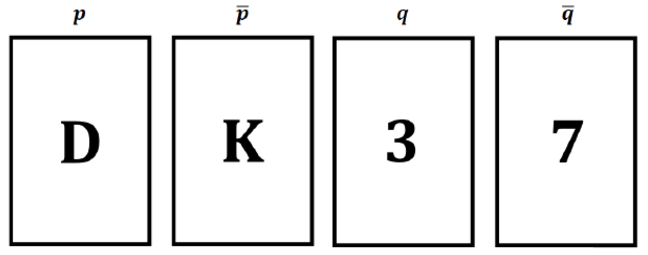
\includegraphics[scale=0.5]{wasonAbstract}
\caption{The Abstract case of the Wason Selection Task}
\end{center}
\end{figure}

The Abstract case of the WST presents the subject with four cards on a table. Their face-up sides read $D, K, 3,$ and $7$. They are asked which cards must be turned over to test the rule:

\begin{center}
``If there is a $D$ on one side of the card, then the other side shows $3$."
\end{center} 
Using classical logic, it is easy to see that turning $D$ to find anything but $3$ would invalidate the rule, as would turning $7$ and finding a $D$. Thus these two cards must be turned to check the rule. However, human subjects very seldom choose this classical answer set and instead overwhelmingly prefer to turn $D$ and $3$. Table~\ref{tbl:can} shows the most common card selection sets for participants.

A great many cognitive theories have been applied to these results, with varying degrees of success \cite{ragni2017formal}. This paper will focus on the WCS interpretation of the task provided by \citep{ragni2017wason}. This approach assumed an initial knowledge base containing only the rule $3 \leftarrow D$.

To illustrate this interpretation of the task we shall use the WCS to examine each of the four cards individually and see what conclusions can be drawn.

When $D$ is observed:

\[
KB = \{3 \leftarrow D, D\leftarrow \top \}
\]

However, at this point, the authors introduce the concept of an abnormality as discussed in \citep{ragni2017formal}. Now, the rule holds only provided that some abnormal even does not occur.

\[
KB_D = \{3 \leftarrow D \land \lnot ab_1, D \leftarrow \top, ab \leftarrow \bot \}
\]

\[
wcKB_D = \{3 \leftrightarrow D \land \lnot ab_1, D \leftrightarrow \top, ab \leftrightarrow \bot \}
\]

The authors also require that, to validate the rule, it must be evaluated after the semantic operator is iterated. Table~\ref{tbl:dcard} shows the result of repeatedly applying the semantic operator to $KB_D$. 

\begin{table}
\begin{center}

\begin{tabular}{ c c c }
 \textbf{Iteration} & \textbf{$\top$} & \textbf{$\bot$} \\ 
 0 &  &  \\  
 1 &  $D$ & $ab$  \\  
 2 &  $D$, $3$ & $ab$  
\end{tabular}
\caption{Applying the Weak Completion Semantics to the $D$ card of the WST.}
\label{tbl:dcard}

\end{center}
\end{table}

When the $K$ card is observed:

\[
KB_K = \{3 \leftarrow D \land \lnot ab_1, K \leftarrow \top, ab \leftarrow \bot \}
\]

\[
wcKB_K = \{3 \leftrightarrow D \land \lnot ab_1, K \leftrightarrow \top, ab \leftrightarrow \bot \}
\]

Table~\ref{tbl:kcard} shows that not enough information can be obtained using only the semantic operator to evaluate the rule $D \leftrightarrow 3$. This is identical to the case for the $7$ card.

\begin{table}
\begin{center}

\begin{tabular}{ c c c }
 \textbf{Iteration} & \textbf{$\top$} & \textbf{$\bot$} \\ 
 0 &  &  \\  
 1 &  $K$ & $ab$  \\  
 2 &  $K$ & $ab$  
\end{tabular}
\caption{Applying the Weak Completion Semantics to the $K$ card of the WST.}
\label{tbl:kcard}

\end{center}
\end{table}

When the $3$ card is observed:
\[
KB_3 = \{3 \leftarrow D \land \lnot ab_1, 3 \leftarrow \top, ab \leftarrow \bot \}
\]

\[
wcKB_3 = \{3 \leftrightarrow D \land \lnot ab_1, 3 \leftrightarrow \top, ab \leftrightarrow \bot \}
\]

In this case, something odd happens. Even though the WCS framework a outlined is not able to deduce anything about the truth value of the variable $D$, participants still very often chose to turn this card. In \cite{breu2019weak} we argue that this may be a result of implicit \textit{abduction}. That is, that the participant subconsciously attempts to identify any possible way in which $3 \leftrightarrow D \land \lnot ab$ could hold when $3=\top$ and $ab=\bot$. The only way for this rule to hold would be for $D$ to be true too:

\begin{table}
\begin{center}

\begin{tabular}{ c c c }
 \textbf{Iteration} & \textbf{$\top$} & \textbf{$\bot$} \\ 
 0 &  &  \\  
 1 &  $3$ & $ab$  \\  
 2 &  $3$ & $ab$  
\end{tabular}
\caption{Applying the Weak Completion Semantics to the $K$ card of the WST.}
\label{tbl:3card}

\end{center}
\end{table}

Now, using Table~\ref{tbl:3card} one can see that $3$ is set to true, the abnormality is set to false, and $D$ has been assumed via abduction. Following \L ukasiewicz logic these assignments are sufficient to evaluate $3\leftarrow D \land \lnot ab$ to $\top$. This the subject will conclude to turn the card.

This simple interpretation of the WST using the WCS and using or not using abduction is sufficient to achieve the most common (general) reasoning of participants. It does not however explain any of the other deviant cases which are observed in Table~\ref{tbl:can}. Why, for example, should it be considered accurate if it gives no information about the classically accurate choice of the $D$ and $7$ cards, chosen by 19 participants, a significant portion? Instead, consider how these aberrant reasoners could be modelled. Perhaps they use extra computational steps or omit steps? This author has previously shown that the WCS is able to model these individual reasoners \citep{breu2019weak} by including two simple processes: Abduction and Contraposition. By including these two processes, and stochastically controlling when they are activated or silenced, it has been shown that not only is this extended framework able to model the major cases of the WCS, but very close approximations to empirical results can also be drawn.

As discussed above, Abduction can be used when the rule under consideration evaluates to unknown. It uses fixing of remaining free varibles to determine if any combination of these can validate or falsify the rule. In the case we have discussed, only fixing $D = \top$ will validate the rule.

Contraposition explicitly makes use of \textit{modus tolens}, usually assumed to be silenced in human cognition to derive certain canonical cases in the WST. In particular, for the card $7$, the logic program:

\[
KB_7 = \{3 \leftarrow D, 7 \leftarrow \top \}
\]

is extended with the rule $\lnot D \leftarrow \lnot 3$, which itself simply means $K \leftarrow 7$ for our restricted domain. 

\[
KB_7 = \{3 \leftarrow D, \lnot D \leftarrow \lnot 3, 7 \leftarrow \top \}
\]

Adding abnormalities yields:

\[
KB_7 = \{3 \leftarrow D \land \lnot ab_1, \lnot D \leftarrow \lnot 3 \land \lnot ab_2, 7 \leftarrow \top, ab_1 \leftarrow \bot, ab_2 \leftarrow \bot \}
\]

After weakly completing:

\[
KB_7 = \{3 \leftrightarrow D \land \lnot ab_1, \lnot D \leftrightarrow \lnot 3 \land \lnot ab_2, 7 \leftrightarrow \top, ab_1 \leftrightarrow \bot, ab_2 \leftrightarrow \bot \}
\]

Applying the semantic operator then yields:

\begin{table}
\begin{center}

\begin{tabular}{ c c c }
 \textbf{Iteration} & \textbf{$\top$} & \textbf{$\bot$} \\ 
 0 &  &  \\  
 1 &  $7$ & $ab_1$, $ab_2$  \\  
 2 &  $K$, $7$ & $D$, $3$, $ab_1$, $ab_2$  
\end{tabular}
\caption{Applying the Weak Completion Semantics and Contraposition to the $7$ card of the WST.}
\label{tbl:7cont}

\end{center}
\end{table}

\begin{figure}
\centering \includegraphics[scale=.6]{wstcano}
\caption{Using the abduction and contraposition extensions to derive all four canonical cases.}
\label{fig:wstcano}
\end{figure}



Table~\ref{tbl:7cont} shows the result of applying the semantic operator to the resulting knowledge base. From this, it is possible to deduce that the card $7$ must be turned. Figure~\ref{fig:wstcano} illustrates the use of these extensions to derive all four of the canonical cases of the WST.

@TODOrewritewholesectionintermsofpq

\section{More}

\chapter{Sequential Cognition Processes}
\section{SCPs: An Intuitionist Description} \label{ssec:intu}
\begin{figure*}
\begin{subfigure}{.35\textwidth}
  \centering
  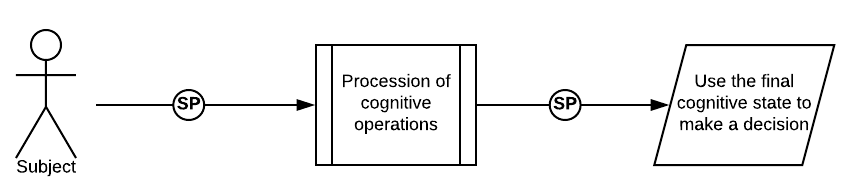
\includegraphics[width=0.97\linewidth]{general}
  \caption{Unrestricted SCP.}
  \label{fig:scp_general}
\end{subfigure}%
\begin{subfigure}{.65\textwidth}
  \centering
  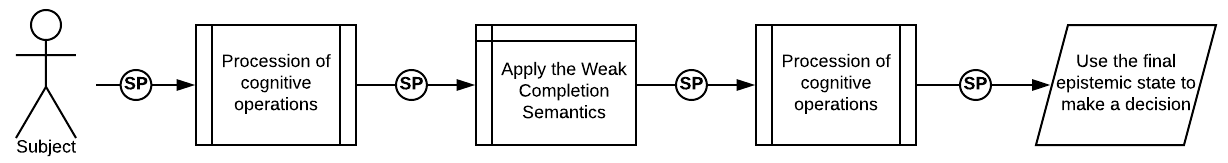
\includegraphics[width=0.97\linewidth]{generalWCS}
  \caption{WCS guaranteed to occur.}
  \label{fig:sfig2}
\end{subfigure}
\caption{The most general description on an SCP with and without guaranteeing the WCS is applied at least once. An agent transitions from one epistemic state to another and then uses it to make a decision. $SP$ nodes indicate state points.}
\label{fig:scp_generalWCS}
\end{figure*}

Although there is evidence that the brain can perform several simultaneous operations when considering a task (such as when considering an image \citep{sigman2008brain}, the SCP framework assumes that at some points in reasoning about a given task, the mental processes of the agent converge to a set of epistemic states, called a \textit{state point}. Whatever happens between these points of convergence can contain any number of parallel processes. The collection of processes that occur between any two state points in a reasoning task is called a \textit{cognitive operation}. It follows that any cognitive operation is valid as long it takes a set of epistemic states as input and produces a set of epistemic states as output. Figure~\ref{fig:scp_general} describes an SCP that is powerful enough to model any cognitive task that involves an epistemic state transition. However, it does not provide any useful information; the nature of the processes followed is completely undescribed. Suppose, instead, that some cognitive task is being modelled, and that researchers have reason to believe that The Weak Completion Semantics should play a part in their model. Under this new restriction, and assuming a sufficiently expressive epistemic state, Figure~\ref{fig:scp_general} is still an accurate model of the process, but now so is Figure~\ref{fig:scp_generalWCS}. By sacrificing some of the ambiguity -- and, thus, expressiveness -- of the model, the information content of the model description has increased. This trade-off is a feature of the SCP framework and finding the right depth of complexity to model the task accurately and still provide meaningful information is more art than science at present. 

\section{SCPs: Mathematical Formulation}
An SCP Task $\Pi=(s_i, \gamma, M)$ consists of an initial epistemic state $s_i$, known goal state $\gamma$, and a known set of cognitive operations $M$. An epistemic state $s_k$ describes all the information available to the agent at state point $k$. The precise contents of an epistemic state should be chosen so that at least some $m \in M$ are able to accept that state as an input. In the case of a system containing only the one complex operation which applies the WCS, one possible epistemic state is $s=(KB,V)$, where $KB$ describes a knowledge base consisting only of rules of the $(head \leftarrow body)$ and $V$ is a mapping of atom names appearing in $KB$ to a truth value in \L ukasiewicz logic ($\top,u, \bot$). In principle this definition will serve for the rest of the paper, but it is extended slightly so that $s_k = (KB,V,R)$ where $R$ is a set of labelled categorization criteria sets (\textit{LCS}). An LCS $ c \in R$ consists of a category name and list of rules and atoms which fit into that category.

A base point is a single epistemic state. A state point $p$ is defined recursively by $p=\{\bar{p} \oplus Q \}$ where $\bar{p}$ is a base point, and $Q$ is a set of state points, and $\oplus$ represents the exclusive-or operation\footnote{$(X \oplus Y) = ((X \cup Y) - (X \cap Y))$ for sets $X$ and $Y$.}. State point containment $\in_s$ for state points $p$ and $q$ is defined recursively as follows:

\[
p \in_s q = \begin{pmatrix} p \in q  & \textrm{True} \\   \exists_{r\in p}p \in_s r = \textrm{True} & \textrm{True}   \\ \textrm{Otherwise} & \textrm{False} \end{pmatrix}
\]

It is never the case that $p \in_s p$.

A cognitive operation $m = (\chi, e), m \in M$ consists of a precondition $\chi$ and a process $e$, such that for an input state point $p$, every base point $\bar{p} \in_s p$ is either accepted as input ($\bar{p} \models m[\chi]$ under whatever definition of $\models$ is used for the complex operation $m$), or else rejected. Every base point is evaluated by the complex operation in isolation (no other base point $\bar{q}$ can affect the output of $m$ on base point $\bar{p}$). To capture the fact that cognitive operation may utilize non-monotonic logic, applying $m$ to an input base point $\bar{p}\in p$ always yields a state point $p'$ (written $J[\bar{p},m]=p'$) which describes all possible resulting epistemic states that can be generated. 

Applying $m$ to an input state point $p$ is done by replacing every base point $\bar{p} \in p$ with $J[\bar{p},m]$. A cognitive operation is called monotonic if it always yields a base point as an output given a base point input ($J[\bar{p},m]=\bar{p'}$). It follows that the depth of a state point is directly related to the number of complex operations which have been performed in the SCP prior to its occurrence. If a base point does not meet the precondition, it is either ignored completely and not processed (\textit{cruel application}), or passed exactly as is to the next complex operation (\textit{lenient application}). It is worth noting that the type of cognitive states produced as output by $m$ may not be the same as those of the input.

This paper will focus on cases where the type of cognitive state remains constant, but there is no reason in principle that a base point input $s_k = (KB,V,R)$ for the WCS could not be returned as a base point $s_k = (KB,V,R,D)$ where $D$ is a set of default rules usable by cognitive operations that implement Reiter's Default Logic \citep{reiter1980logic}. Future models of human cognition may well rely on background knowledge which draws inferences from multiple types of non-monotonic logics.

An SCP $\pi=(s_i,m_1,...,m_n)$ describes an initial epistemic state (or state point if the input is uncertain) and state point $p_k$ is defined recursively by $p_k = J[p_{k-1},m_k]$. An SCP is called \textit{credulously valid} if $p_n \models \gamma$ for at least one epistemic state in the final state $p_n$. An SCP is called \textit{sceptically valid} if $p_n \models \gamma$ for every epistemic state in the final state. In cases where all operations are monotonic, sceptical validity is the same as credulous validity.
\section{SCPs vs SCP Tasks}
The distinction between SCPs and SCP tasks is fairly straightforward: An SCP task describes a cognitive phenomena that has been observed and details the tools and constraints which may be used to model it; and an SCP is a single solution to the problem described in the SCP task which does not violate conditions outlined in that task.

For a given SCP task there can be many possible SCPs (the question of how to choose the most probable of these candidate SCPs is discussed in Section~@TODOref), or no possible SCPs at all.

\section{Epistemic States}
The choice of epistemic state is dependent on the properties that are known or suspected to be true for the cognitive task as a whole. For example, a researcher working on drawing inferences using Propositional Logic can be certain that any SCP they create should be expressive enough to pass a knowledge base to a cognitive operation. Thus, it might suffice to simply define $s_i=(KB)$ where $KB$ is a set of propositional rules. By contrast, a researcher using the WCS requires a system capable of both communicating a set of rules to the next complex operation, and of describing the results of repeated applications of the semantic operator. It might seem intuitive to simply keep the epistemic state used for the propositional case and to use a non-complex operation function on the weakly completed program to find the least model. And, though this approach works for many examples, it makes it impossible to perform further processing in the SCP \textit{after} applying the semantic operator. What if the conclusion drawn was meant to form part of the background knowledge of another process? In practice using $s_k=(KB,V, R)$, where $V$ is a set of (variable name, value pairs) and $R$ is a categorization variable, is able to model all aspects of the WCS, including information related to the least model. 

The final property of a cognitive operation that needs to be discussed is how it is able to interact with the categorization variable $R$. Imagine a case drawn from \cite{saldanha2017weak} where the difference between creating abnormalities for obligate and factual conditionals is discussed. The intuition behind the authors' work can be summarised by saying that there are two different types of conditional statement, those that \textit{have to be} true, and those that are \textit{usually} true. If it rains $r$, I will normally take my umbrella $u$ (in the absence of something abnormal happening, like a plague of umbrella-stealing gnomes). This a statement that is usually true, but some things are definitely true. For example, when it rains, water has to fall out of the sky $s$. This is an essential property of rain, not subject to abnormalities. Thus one useful set of categorizations for researchers seeking cosmic knowledge of weather patterns may be: $R=\{obligate: \{u \leftarrow r\}, factual: \{s \leftarrow r\} \}$. With these labels we might then expect that the process followed by the operation $m \in M$ which creates abnormalities would treat the two conditionals in $KB$ differently, because of their assignments in $R$. $R$ then is a way of expressing meta information to the cognitive operations, and it is completely possible that some operation $m_k$ might change $R$ is such a way that future operation $m_{k+l}$ produces different output. This is a technique we will exploit in several examples in this paper.

As yet, there are no definite rules for creating an epistemic state, but Albert Einstein's famous advice from 1950 still rings true: ``Everything should be made as simple as possible, but no simpler.'' The ideal epistemic state is one that enables every reasonable cognitive operation in $M$ that might help model the problem, without adding superfluous functionality that might render searching the SCP space infeasible.

\section{State Points}
\section{Cognitive Operations}
The set of possible complex operations $M$ determines many attributes of the achievable final state point $p_n$. If every $m \in M$ is monotonic, then $p_n$ will be monotonic. If some cognitive operation is computationally complex or produces a very large number of output state points, then search using that base point becomes less efficient. If some complex operation $m'$ (such as weakly completing) is known or believed to occur in the SCP, then a restriction on the cognitive states exists such that either the initial state is of a format suitable as input for $m'$, or there exists another cognitive operation which is able to output a state point which contains base points of a suitable format.

More abstractly, the set of cognitive operations should be well-founded in the literature. The set of possible complex operations is infinite and an SCP only meaningfully describes human cognition when it contains cognitive operations that have been justified empirically (\textit{modus ponens-modus tolens} asymmetry, suppression, denial of the antecedent, etc.). 

\section{Pre-conditions and Effects}
\section{The Categorization Variable}
\section{Search in SCP-Space}
\subsection{De-Novo SCP Searching}
\subsection{Insertion Search}

\chapter{Cognitive Operations: The Cognitive Toolbox}
%reference that paper that shows the improvements in machine learning
\section{Overview}
As discussed in Section~\ref{ssec:intu},and illustrated in Figure~@TODOref the simplest imaginable description of sequential human cognition consists of a single step transforming the initial task information (along with background information) into an epistemic state that can be externally interpreted to choose a response. Assuming that this single operation $A$ transforms the initial knowledge base $x$ into final state $x'$ which is interpreted by external function $f()$, we can use the shorthand $f(x \longmapsto A)$, where $\longmapsto$ is a function that takes state point $x$ as input and produces a new state point $y$ as output, to summarise this process. 

To understand why this is poor choice of SCP, consider a general limitation of the SCP framework: we can only change the output of an SCP by changing the initial epistemic state, or by inserting/deleting a cognitive operation at an existing state point. Consider a case where the initial epistemic state is immutable. Thus, for $f(x \longmapsto A)$, the only possible changes are: $f(x \longmapsto \bar{B} \longmapsto A \longmapsto \bar{B})$, $f(x \longmapsto A \longmapsto \bar{B})$, $f(x \longmapsto \bar{B} \longmapsto A)$, $f(x \longmapsto \bar{B})$, and $f(x)$. Where $\bar{B}$ denotes the action of drawing some sequence of random, but valid cognitive state transitions. There is no way to change the operations that occur in $A$. Thus, even though Figure~@TODOref may be an appropriate model for the general reasoner of a given task, it imposes the explicit assumption that all other test subjects who achieved differing results, achieved only by completely ignoring the black-box process the general reasoners used, or else by inserting new operations only at the very start or end of the processing task. We will see an example in Section~@TODOref of cases where assumptions like that are simply not reflected by empirical data. 

Instead of using a single black-box operation to describe all cognition, it follows logically to use multiple smaller black box operations, each connected by a state point. Using this interpretation, cognitive operations for the general reasoner should be as extensive as possible, provided that they do not force implausible changes to describe deviant users or when used in other cognitive tasks. Figure~@TODOref captures this intuition as it applies to the Weak Completion Semantics. Indeed, as a non-monotonic logic that is already explicitly divided into discrete steps in the literature @TODOref, obvious candidate cognitive operations present themselves.

It is worth noting that this increased ability to model deviant reasoners comes at the cost of forcing more state points into the SCP being used.

The remainder of this section is devoted to expressing the exact properties, limitations, and concrete descriptions of cognitive operations.

@TODOlayout

\section{Cognitive Operation Space}
%then SCP space is cog op space size ^^ scp length
In principle, the number of cognitive operations available for use in an SCP is unlimited. We denote the space of all cognitive operations $\Omega$, and the space of all sequences $(A_0 \longmapsto ... \longmapsto A_n)$ with $\Omega^*$. There cannot and never will be an exhaustive search procedure to evaluate every possible way of manipulating an epistemic state (Proofs~\ref{proof:infiniteSCPs} and \ref{proof:infiniteSCPLength} illustrate the existence of valid SCPs for infinitely many different cognitive operations and valid SCPs of any length, respectively). However, there are ways of limiting the number of allowable cognitive operations. Lemma~\ref{lem:uniredundant} defines those cases in which there is redundancy in the set of all possible cognitive operations, Lemma~\ref{lem:taskredundant} focuses this concept on specific cognitive tasks which are to be modelled using SCPs.

\begin{proof} \label{proof:infiniteSCPs}
There are an infinite number of possible, valid SCPs, that can meet any goal condition $\gamma$ from input $x$ provided that at least one SCP exists that can reach goal condition $\gamma$ from input $x$.
\begin{enumerate}
\item There exist infinitely many cognitive operations $T \in \Omega$ which add a new variable from the set of all possible variable names $p \in P$.
\item There exist infinitely many cognitive operations $V \in \Omega$ which remove a variable from the set of all possible variable names  $p \in P$.
\item It follows that there exist infinitely many pairs $(T_i \in T, P_i \in P) \in W$ where $T_i$ adds a variable $p \in P$ to the resulting state point, and $V_i$ removes that variable from the resulting statepoint.
\item Then $f(x \longmapsto A) = f(x \longmapsto T_i \longmapsto V_i)$
\item Thus it follows that if $f(x \longmapsto A)\models \gamma$ then $f(x \longmapsto T_i \longmapsto V_i)\models \gamma$ for all $(T_i \in T, P_i \in P) \in W$.
\end{enumerate}
\end{proof}

\begin{proof} \label{proof:infiniteSCPLength}
If there exists an SCP which meets goal condition $\gamma$ of length $n$, then there exists an SCP that meets goal condition $\gamma$ of length $n+k$ where $k$ is any natural number.
\begin{itemize}

\item Proof~\ref{proof:infiniteSCPs} states that if $f(x \longmapsto A)\models \gamma$ then $f(x \longmapsto T_i \longmapsto V_i)\models \gamma$ for all $(T_i \in T, P_i \in P) \in W$.
\item Let $X$ be a partial SCP of the form $X=T_0 \longmapsto V_0 \longmapsto ... \longmapsto T_N \longmapsto V_{N}$ where $(V_i, T_i) \in W$
\item For odd lengths:
\begin{itemize}
\item  It follows that if $f(x \longmapsto A)\models \gamma$ then $f(x \longmapsto A \longmapsto \textrm{exp}(X))\models \gamma$, where $\textrm{exp}$ denotes the substitution of $X$ for its constituent parts.
\item Because $X$ always contains an even number of cognitive operations, then the length of the resulting SCP must be $n' = 1+v$ where $v$ is any even number.
\end{itemize}
\item For even lengths:
\begin{itemize}
\item Notice that $f(x \longmapsto A \longmapsto \textrm{exp}(X) \longmapsto X) \models \gamma$.
\item A appending $\longmapsto X$ to adds one to the length of any SCP.
\item Because we have shown that a suitable SCP of any odd length exists $n'>=n$, it follows that a suitable SCP of any even length $n'>n$ exists.
\end{itemize}
\end{itemize}

\end{proof}

\begin{lemma} \label{lem:uniredundant}
Given a cognitive operation sequence $A \in \Omega^*$, and external function $f()$, $A$ is redundant redundant iff one of the following holds:
\begin{itemize}
\item $(x \longmapsto B \longmapsto C) \models x'$ and $(x \longmapsto A) \models x'$ for every viable epistemic state $x$, $B \in \Omega^*$, $C \in \Omega^*$. 
\item $x \longmapsto A \models x$ for every viable epistemic state $x$.
\item $f(x \longmapsto B)=c$ for all $B \in \Omega^*$, where $c$ is a constant external decision.
\end{itemize}
\end{lemma}

\begin{lemma} \label{lem:taskredundant}
Given a limited set of cognitive operations $M=\{A_0, ..., A_n\}, A_x \in \Omega^*$, and external function $f()$, $A \in M^*$ is task redundant iff one of the following holds:
\begin{itemize}
\item $(x \longmapsto B \longmapsto C) \models x'$ and $(x \longmapsto A) \models x'$ for every viable epistemic state $x$, $B \in M^*$, $C \in M^*$. 
\item $x \longmapsto A \models x$ for every viable epistemic state $x$.
\item $f(x \longmapsto B)=c$ for all $B \in M^*$, where $c$ is a constant external decision.
\item There exists no epistemic state $x$ and sequences $B, C \in M^*$ such that $f(x \longmapsto B \longmapsto A \longmapsto C)$ is a valid SCP.
\end{itemize}
\end{lemma}

The total number of possible non-trivial SCPs of length $n$ for an SCP Task is given by $(|M|^L - R)$ where $|M|$ is the number of elements in the set of cognitive operations $M$, $L$ is the length of the SCP, and $R$ is the number of possible non-overlapping task redundant SCPs for the task. @TODOdefineOverlappingRedundantSCPs


\section{A Limited Set of Allowable Operations}
In practice it is impossible compute the set of all candidate SCPs when the set of allowable cognitive operations $M$ in a planning task is $\Omega^*$ or even $\Omega$. Without a length constraint Proof~\ref{proof:infiniteSCPLength} shows that it is not even possible to compute all possible SCPs for many SCP tasks with a finite set of allowable operations. Table~\ref{tbl:solutionSpace} summarises the properties of solution space under different SCP task conditions.

\begin{table}
\begin{center}

\begin{tabular}{ c c c c}
 \textbf{$M$} & \textbf{Finite Length Constraint} & \textbf{Finite Solution Space} & \textbf{Guaranteed Solution}\\ 
 $\Omega^*$ & None & \text{\sffamily X} & \checkmark \\ 
 $\Omega^*$ & Yes & \text{\sffamily X} & \checkmark \\ 
 $\Omega$ & None & \text{\sffamily X} & \checkmark \\ 
 $\Omega$ & Yes & \text{\sffamily X} & \checkmark \\  
 finite &  None & not guaranteed & \text{\sffamily X}\\  
 finite &  Yes &  \checkmark & \text{\sffamily X}
\end{tabular}
\caption{Solution space considerations of SCPs tasks as determined by length constraints and choice of cognitive operations.}
\label{tbl:solutionSpace}

\end{center}
\end{table}

\subsection{A Limited Set of Cognitive Operations}\label{ssec:limCogOp}
Readers should recognize that using the space of all possible cognitive operations for $M$ results in a computationally impossible task. No matter the other conditions imposed there will be infinitely many solutions to the given SCP task which satisfy $f()$.

But, beyond being just computationally infeasible, there are more empirical and philosophical objections to this approach. The first is that the human brain itself does not have infinite processing or space capabilities and so any model which allows for unrestricted data sizes in the set of allowable cognitive operations $M$ or in the number of resultant state points $M$ is not biologically well-founded\footnote{Because $\Omega$ is the set of all possible cogntive operations there must be at least one $m \in M$ such that, for any given input $x$, $x\longmapsto m$ results in a state point of size greater than the capacity of any storage system to hold.}. 

The second considerations is that there is considerable evidence in the literature that many problems can be modelled using logical frameworks which describe cognitive behaviour across a variety of tasks @TODOref. These frameworks reflect a more generally philosophy in cognitive psychology which is the idea of consistent cognitive motifs in reasoning. Using an infinite $M$ shows no discrimination at the time of task-formulation between those operations for which there is significant evidence and those which are fundamentally improbable.

\subsection{A Limited SCP Length}
As discussed in Section~\ref{ssec:limCogOp}, the human brain is constrained by a set of physical computational and storage limitation. In all case except those which are trivial or repetitive it would be computationally infeasible for the human mind to mimic an infinitely long SCPs. For this reason, SCPs of infinite length, though possible in a mathematical formulation, tend violate the spirit of the SCP Framework which is to \textit{accurately} model human cognition processes, not simply their conclusions.

It is worth noting that SCPs containing infinite loops can exist and can be evaluated at any time point $n$, they simply cannot be evaluated in their entirety.

\section{Purpose-Selected Cognitive Operations}
\subsection{Overview}
\subsection{Initialisation}
The initialisation cognitive operation (\texttt{init}) is always the first operation in an SCP. Thus, unlike every other cognitive operation, \texttt{init} has no prior cognitive operation from which to draw an epistemic state. Instead, it creates an epistemic state that reflects the initial inferential rules and variable assignments known by the agent. These rules and assignments are drawn from two distinct sources:
\begin{itemize}
\item \textbf{The initial interpretation of the task given}: in the case of the Suppression Task, for example, this rule corresponds to the given rules about Alice and the Library.
\item \textbf{Background information}: though this knowledge base is as large as every fact and inferential rule by known the participant, no computational is lost by only showing those facts and inferential rules that directly relate to the task in question\footnote{The question of precisely \textit{how} to sift through that enormous amount of information and select appropriate knowledge for the task at hand is an open problem.}.
\end{itemize}

In many ways it could be argued that the \texttt{init} operation is simply an aggregate cognitive operation that each encodes either a variable or rule insertion into the epistemic state (@TODOfig). The one caveat to this interpretation is that there must still be some first cognitive operation which takes no input and produces an epistemic state of suitable structure as output.

Because it is actually used as a shorthand for whatever sequence of sub-operations is needed to represent the initial epistemic state \texttt{init} is the only cognitive operation which differs on a task-by-task and a reasoner-by-reasoner basis. Every other cognitive operation is a uniquely-named pipeline whose internal structure is fixed for any task in which it appears.

\subsection{Variable Insertion}


\subsection{Variable Deletion}
\subsection{Variable Silencing}
\subsection{Variable Fixation}
\subsection{Adding Abnormalities}
\begin{figure} 
\begin{center}
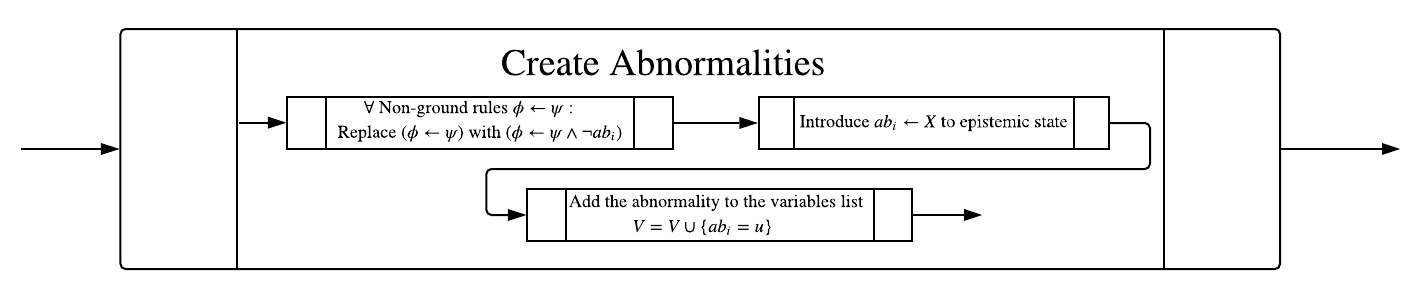
\includegraphics[width=\linewidth]{abnormalitySCP}
\end{center}
\caption{One possible formulation of a cognitive function to add abnormalities to variables. This formulation follows the intuition of Appendix~@TODOref.}
\label{fig:addAB}
\end{figure}

One of the most obvious candidates for a cognitive function that has evidence across a wide swathe of the cognitive literature (@TODOrefAFewPapers) is the idea of adding an abnormality variable to a problem that does not appear in the initial formulation of that problem. In Section~@TODOref and Section~@TODOref we discussed the idea of abnormalities as licenses for implication. The fact that we can point to several tasks in which an abnormality variable is added after formulation provides compelling evidence that creating these abnormality variables is a well-founded cognitive process that should be included in any comprehensive formulation of $M$. Figure~\ref{fig:addAB} shows one possible formulation of the \texttt{addAB} function for adding abnormalities to a knowledge base of the form $s=(KB,...)$ where $KB$ is a set of rules, and $V$ is a set of (variable name, variable value) pairs.



\subsection{Weakly Completing}
\begin{figure} 
\begin{center}
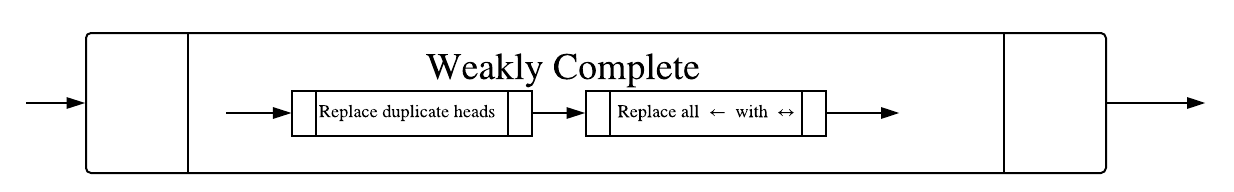
\includegraphics[width=\linewidth]{weaklycompleteSCP}
\end{center}
\caption{One possible formulation of a cognitive function to weakly complete a set of rules. This formulation follows the intuition of weak completion outlined in Section~@TODOsec.}
\label{fig:weaklycompleteSCP}
\end{figure}

Weak completion is an essential part of the WCS. Under the assumption that the WCS is a valid representation of human cognition in at least one scenario, any comprehensive set of cognitive operations $M$ must be able to mimic the Weak Completion of a knowledge base. Figure~\ref{fig:weaklycompleteSCP} how this can be achieved for any epistemic state of the form $s=(KB,...)$.


\subsection{Semantic Operator}
\begin{figure} 
\begin{center}
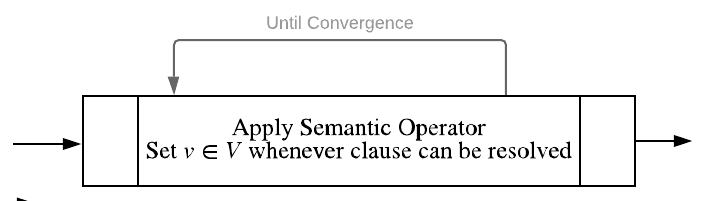
\includegraphics[width=\linewidth]{semanticOperatorSCP}
\end{center}
\caption{One possible formulation of a cognitive function to apply the semantic operator a congnitive state by temporarily setting all variables in $V$ to any value that can computed using the semantic rule in Equation~@TODOref. This process is repeated until $V$ is no longer updated. @TODOredoThisDigramToShowActualProcess}
\label{fig:semanticOperatorSCP}
\end{figure}

Another essential step in the WCS, the semantic operator is used to assign all variables to either True or False (explictly), or to Unknown (implicitly). Figure~\ref{fig:semanticOperatorSCP} illustrates one way in which this cognitive operation can be implemented for any epistemic state of the form $s=(KB,V,...)$.



\subsection{Default Inferencing}
If we assume that Reiter's default logic is a valid model of cognition for at least one task, it follows that an comprehensive formulation of $M$ must encode a cognitive operation for drawing inferences from a set of default rules. Figure~@TODOref illustrates the procedure for drawing such inferences from an epistemic state state of the form $s=(KB,V,D)$ where $KB$ is a set of inference rules, $V$ is mapping of variable names onto variable values, and $D$ is a set of default rules of the form $\frac{condition:exception}{conclusion}$ @TODOrewriteEquationWithStandardSymbols.

\section{Cognitive Operations as Aggregates}
%talk about combining existing cognitive operations for which there is strong evidence
An obvious and interesting idea follows from Proof~\ref{proof:aggregateValid} which is the idea of finding well-founded, uninterrupted epistemic operation sequences which are effective in modelling a variety of tasks and representing them as a single epistemic operation. We call this approach \textit{aggregating}, and it draws inspiration from recent advances in the field of reinforcement learning @TODORef in which simple tasks previously achieved are used as allowable actions when attempting to solve complex tasks.

This approach introduces the desirable property of shortening the total length of the SCP for a given set of cognitive tasks. However, it is evident from Proof~\ref{proof:aggregateExpressiveness} that any SCP task in which an aggregated subsequence of operations replaces those individual operations in $M$ may be less expressive than the same formulation in which the aggregated operations are still present.

\begin{proof} \label{proof:aggregateExpressiveness}
Given a cognitive task $\Pi=(x,f(), M, \gamma)$ in which $M=\{A_0,...,A_n\}$ and a second cognitive planing task $\Pi'=(x,f(),M')$ in which $M'= M \smallsetminus \{A_k,...,A_m\} \cup A'$, where $A'=(A_k \longmapsto... \longmapsto A_m)$ is a cognitive sequence containing some ordering of the other operations in $(\Pi \smallsetminus \Pi')$, $\Pi'$ is as expressive or less expressive than $\Pi$.

\item No more expressive:
\begin{itemize}
\item If $\pi' = (x\longmapsto A_p \longmapsto ... \longmapsto A' \longmapsto ... \longmapsto A_q)$ and $f(\pi)$ is a solution to $\Pi'$.
\item Let $\pi'' = (x\longmapsto A_p \longmapsto ... \longmapsto [A'] \longmapsto ... \longmapsto A_q)$.
\item Then $f(\pi'')$ is a solution to $\Pi'$ (Lemma~\ref{lemma:substitutionValid}).
\item $f(\pi'')$ is a valid solution to $\Pi$ because $\pi''$ uses only cognitive operations which occur in $\Pi$, $x$ is the initial epistemic state, and $f(\pi'') \models \gamma$. 
\end{itemize}

\item Less Expressive: Proof by counterexample
\begin{itemize}
\item If we assume that $\Pi'$ is strictly as expressive or more expressive than $\Pi$, then there exist no cases in which $\Pi'$ is less expressive.
\item Let $\gamma = \emptyset$, and $f(x)=True$ for all inputs (i.e. is trivially satisfied).
\item Let $x=\{\}$, $M=\{A_0,A_1\}$, $M'=\{A'\}$, $A'=\{A_0\longmapsto A_1\}$.
\item Then solutions of $\Pi$ are $f(x)$, $f(x \longmapsto A_0)$, $f(x \longmapsto A_1)$, $f(x \longmapsto A_0\longmapsto A_1)$ and $f(x \longmapsto A_1\longmapsto A_0)$.
\item Solutions of $\Pi'$ are $f(x), f(x \longmapsto A')$.
\item Thus, $\Pi'$ has fewer solutions that $\Pi$. A contradiction.
\end{itemize}
\end{proof}

@TODOexample?

The use of aggregates then, is a trade-off between sacrificing cross-reasoner accuracy and optimising a set of desirable heuristic properties such as length minimisation.

In many ways this compromise follows the philosophy of cognitive modelling in general. A neuron-by-neuron approach to predicting human behaviour (if one were ever possible) would give us extreme accuracy in modelling any human reasoner, but is too complex to be practical, and even if it were, would provide no abstracted information with which to find common motifs and inferences among reasoners. On the other extreme, modelling reasoners as (\textit{input}, \textit{output}) pairs perfectly captures the average predictions of a population, but proves very inaccurate for unseen individuals. State-of-the-art approaches to cognitive modelling like neural networks and non-monotonic logical frameworks seek generalizations which accurately capture the responses of most reasoners across as many tasks as possible by approximating human motifs in human reasoning and applying across multiple tasks and inputs.

The question of how to generate appropriate complex operation aggregates is a complex problem and is not discussed further in this thesis. It is, however a topic in which the author has significant interest.

\begin{proof} \label{proof:aggregateValid}
Given an SCP $\pi= f(x \longmapsto A_0 \longmapsto ... \longmapsto A_n)$, where $f(x)$ is an external evaluation function, $x$ is a state point, and $A_i \in \Omega$, any subsequence $A'=(A_k \longmapsto ... \longmapsto A_{k+l})$, $(k+l)<n$ of the cognitive operations in $\pi$ is a valid cognitive operation.
\begin{itemize}
\item Given that $\pi$ is a valid SCP, $x \longmapsto A_0$ must, by the definitions discussed in Section~@TODOref result in a valid state point.
\item It follows that $A'$ takes a valid state point as input, because $A_k$ took a valid state point as input.
\item It follows that $A'$ produces a valid state point as output, because $A_{k+1}$ produced a valid state point as output.
\item Therefore, $A'$ is a valid cognitive operation, by the definition in Section~@TODOref.
\end{itemize}
\end{proof}

\begin{lemma} \label{lemma:substitutionValid}
Let $\pi=(x\longmapsto A_0, ..., A', ..., longmapsto A_n)$ be a sequence of cognitive operations drawn from some cognitive task $\Pi=(x, \gamma, f(x), M)$ . And let $\pi'=(x\longmapsto [A_0], ..., A', ..., longmapsto A_n)$ where $[A]$ is the substitution of the aggregate operation $A'$ for $(A'[0]\longmapsto ... \longmapsto A'[t])$ . Then $f(\pi)=f(\pi')$.
\end{lemma}

\section{Epistemic State Structure Changes with Cognitive Operations}
%e.g. going to WCS to Default
\section{Purpose-Built Cognitive Operations}
\subsection{Propositional Logic}
%no requirement of sequence, just exhaustive search
%not computationaly valid, NP-complete is too hard for human brain
\subsection{Weak Completion Semantics}
\subsection{Default Logic}
\section{Two Approaches to Creating Cognitive Operations}
\section{Theoretical Approximation}
%must have empirical basis, but focused on reproducing mechanisms that have been proposed and substantiated in literature
%hand-curated
It seems reasonable that, given our desire to accurately model reasoning in participants, researchers creating cognitive functions for SCPs would choose to limit the set of allowable cognitive operations to those for which there is a sound theoretical basis. The reasons for this choice were discussed in Section~@TODOref.

The first approach to creating cognitive operations we will consider is the use of cognitive operations for which there is already evidence in our existing models of human cognition. This evidence can take a wide variety of forms: it may follow from our knowledge of physics (for example, the impossibility of storing a set of unrelated variables above a certain physical threshold); evolutionary biology (there cannot exist a class of organisms without some kind of reproductive drive); anatomy (there must exist cognitive processes that facilitate voluntary muscle activation); sociology (some neuronal connections seem to restrict the number of close friends a human can maintain @TODOref); or any other field of science. Using this information can allow researchers to predict what cognitive functions may play a role in observed empirical data. 

For the most part, theoretical approximation is a very powerful and well-justified mechanism for determining which cognitive operation could plausibly considered in the cognitive toolbox for a given task. Restricting the space of other cognitive operations which may play a part is also enabled by all the scientific fields mentioned above, complexity theory tells us that humans are unlikely to apply exhaustive classical logic reasoning to a task when the set of variables and rules to be considered is large because of physical limitations related to solving \textit{NP-complete} or harder tasks efficiently.

At present, the foundation of non-monotonic reasoning in cognitive modelling is this theoretical mindset, a well-founded explanation is found by borrowing from a relevent field (often psychology) and then tested against empirical evidence and across multiple cognitive tasks to show evidence that is a reasonable approximation of a mechanism in human cognition.


\section{Empirical Appoximation}
%finding cognitive operations using machine learning
%done by using search techniques to create and explore comparison space
Contrasting theoretical approximation is the field of constrained empirical approximation. Techniques ranging from neural networks and Markov models genetical inspired techniques consistently outperform humans in a huge variety of fields. Drawing on enormous databases of empirical data, modern artificial intelligence researchers have come to view machine learning as the most plausible way to create the first real thinking machine @TODOref.

@TODOfinish

\chapter{Mimicking Non-Monotonic Logics With SCPs}

\section{The Suppression Task}

\section{The Weak Completion Semantics}



\chapter{Modelling Experiments with SCPs}
\section{Overview}
\section{Suppression Task}

\begin{figure*}
\begin{center}
 \centering 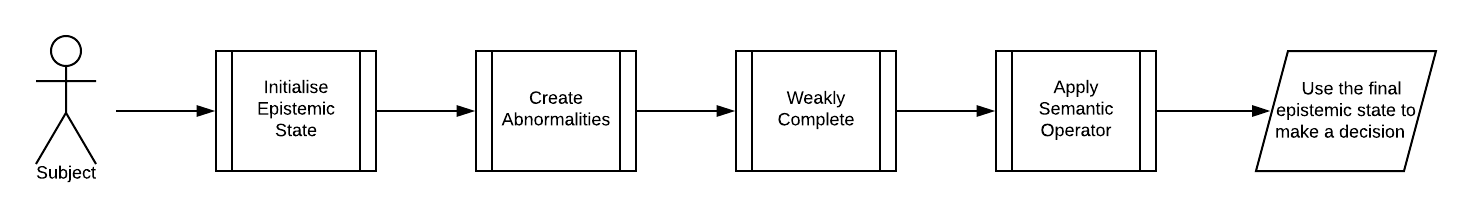
\includegraphics[width=\linewidth]{suppressionSCP_overview}
\caption{A generalised illustration of the WCS in an SCP. }
\label {fig:supoverview}
\end{center}
\end{figure*}

\begin{figure*}
\begin{center}
 \centering 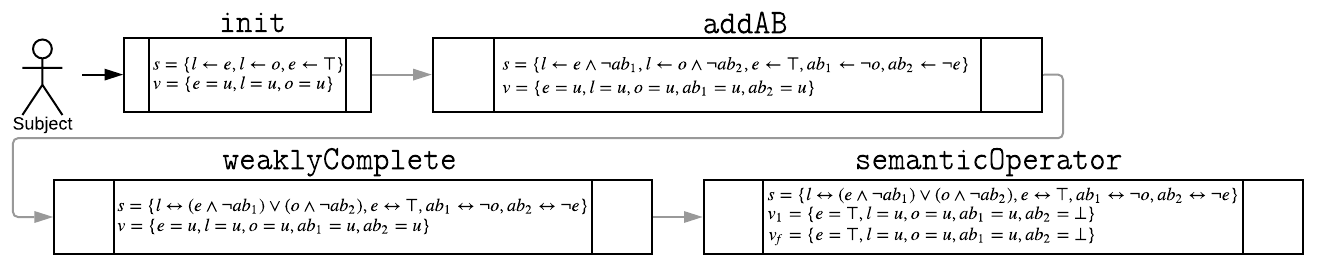
\includegraphics[width=\linewidth]{suppressionSCP_normal}
\caption{The standard case of the Suppression Task, demonstrating the suppression effect. Where the epistemic state in the boxes represents the output of that cognitive operation. $V_f$ represents the assignment of $V$ in the epistemic state in the resulting least model. $V_{i\in \mathbb{N}}$ represents the assignments in $V$ after $i$ iterations of the semantic operator.}
\label {fig:supnormal}
\end{center}
\end{figure*}

Figure~\ref{fig:supoverview} illustrates a generalised SCP to describe the Suppression Task as a series of sequential steps directly mirroring the discrete steps outlined in Section~\ref{sec:sup}, each cognitive operation passing information to the next process\footnote{It is important to note that a diagram like this is valid for \textit{any} cognitive modelling task because any process may be arbitrarily complex and non-sequential. and so the overall linear process of (actor, complex decision, observed results) is always valid for retroactive modelling, and at least as powerful as the non-monotonic logic framework it uses for modelling.}. To model the SCP the implicit sequence of operations in the Suppression Task is systematized and refined into a set of complex operations. Further we introduce an initial epistemic state $s_i=(KB,V,R)$. One interpretation of the requirements of the suppression task $\pi=(s_i,\gamma,M)$ using SCPs and the WCS is as follows: 
 
 
 
 


\[s_i=\{KB_i, V_i, R_i\} \]
\[KB_i=\{e \rightarrow l, \top \rightarrow e, o \rightarrow l\} \]
\[V_i=\{e:u, l:u, o:u\} \]
\[R_i=\{\} \]
\[
\begin{split}
M= \{\texttt{init}, \texttt{addAB}, \texttt{WeaklyComplete}, \texttt{semanticOperator}\}
\end{split}
\]
\[\gamma = (l\models \top) \textrm{ or } (l \models \bot)\]

%@TODO change semanticOper to semanticOperator without line overflowing 

where all cognitive operations require as input and produce as output a state point $p$ where every ground point $\bar{p} \in_s p$ is of format $\bar{p}=(KB,V,R)$; \texttt{init} is always the first cognitive operation and adds the initial variables and rules to epistemic state; \texttt{addAB} adds abnormalities to the current epistemic state using the procedure described in Algorithm~\ref{alg:addAbnormalities} (but now also adds those abnormalities to the variable list of the epistemic state); \texttt{WeaklyComplete} weakly completes the knowledge base of the current epistemic state; and \texttt{semanticOperator} returns an epistemic state that leaves the knowledge base unchanged but updates the variables of that state to return the least model of the epistemic state. \texttt{semanticOperator} follows the same logic seen in Section~\ref{ssec:wcs}, but directly updating $V$ after each iteration of the semantic operator, instead of the externalised variable set $J$. Thus, we ensure that the output state point is able to communicate the result of applying the semantic operator without any structural changes to the epistemic states it contains. As an additional feature of the \texttt{semanticOperator} cognitive operation, if there exists a labelled set in $R$ called $fixed$, then the semantic operator will not set the value of any $v \in fixed$ in the variables list $V$. The goal $\gamma$ states that $l$ should no longer be mapped to unknown in the final epistemic state.



Treating Figure~\ref{fig:supoverview} as an SCP, we observe the sequence of output states seen in Figure~\ref{fig:supnormal}. Note that in the final state $l$ remains mapped to $u$, meaning that the suppression effect is demonstrated.

\subsection{Extending the Suppression Task with SCPs}
The previous example merely showed that SCPs are suitable for modelling the suppression task. In this example we consider one of the most powerful characteristics of SCPs, the ability to model unusual results as deviations from general reasoning. In the original Suppression Task Experiment examined in Section~\ref{sec:sup}, a significant portion of people still believed that she would study late in the library, even though the majority suppressed the inference. Several possible explanations are intuitive, the first and simplest, is the assumption that the reasoner is using classical logic and drawing the classical conclusion. However, what if that is not the case? What if they do reason in exactly the same way as the other reasoners, except for one or two small deviations?

In order to model these non-general reasoners, we consider two possible deviations that could explain the classical result of the Suppression Task: \textit{variable deletion}, and\textit{ variable fixation}. Both of these operations will be discussed in a way that may seem overly prosaic, but it is done to reinforce that we might, reasonably, expect these cognitive operations to occur in day-to-day human cognition.

\subsection*{Variable Deletion} \label{ssec:variableDeletion}
Consider the sequence of numbers: 1, 44, 27, 8, 0 , -4, 6, 7, 346, 7, 74, 7, 234, -55, 2.4, 18. Now without looking back at the numbers, ask yourself some questions: how many numbers were there? Were any of them prime? How many numbers were repeated? In all probability you are not entirely sure. This simple thought experiment provides support for our first extension, the idea that variables can be ``forgotten", that is, that information that existed in the knowledge base at one point in time might no longer exist at a later timepoint. 

This is not the only imaginable case where a variable might be removed from the knowledge base of the person being modelled. The size of the knowledge base used for cognitive modelling is always implicitly restricted to relevant variables. Only those variables whose values might reasonably be expected to affect the final conclusions drawn with regard to the research question should be considered. Finding which variables and rules are relevant is, however, non-trivial. For another real-life example, imagine a mystery novel: Three hundred pages of plot descriptions, character actions, and dialogues. In a good murder mystery novel every piece of information that reveals the killer's identity is hidden in the story itself, yet we do not hold every fact and interaction in the book in our epistemic model of the book, so discerning the identity of the killer remains a mystery until the last page. But when the mystery is solved, many details that we internalised while reading (and recall in retrospect) suddenly make the conclusion seem obvious. We have not forgotten this information, we had merely incorrectly deemed it irrelevant at the time and ignored it in our cognitive processing.

The exact details of how to delete a variable from a knowledge base are non-trivial, and there is no best practice for doing so. But in simple cases the process can be intuitive. Let \texttt{delete} be a complex operation. \texttt{delete} takes as input any state point and is applicable for any ground point $\bar{p}$ with variable list $V \in \bar{p}$ and categorization variable $R$ with ($delete:V_{del}) \in R$, where $V_{del}$ is the set of variable names to delete. For every $v \in V_{del}$ remove all rules from $KB$ that have $v$ as body or head of the clause, and remove $v$ from $V$. Then remove $delete$ from $R$.

In the case of the Suppression Task we argue that one cognitively valid reason for drawing the classical conclusion to the task may be forgetting (or disregarding) the variable $o$. Figure~\ref{fig:supmod} illustrates this case, and shows how the insertion of a complex operation can completely change the final epistemic state.

\begin{figure*}
\begin{center}
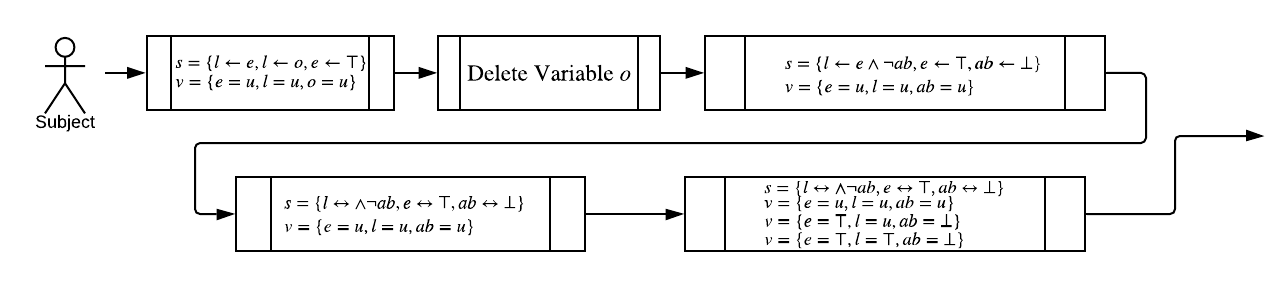
\includegraphics[width=0.85\linewidth]{suppressionSCP_mod}
\end{center}

\caption{The Suppression Task in which the additional operation of deleting the variable $o$ occurs.}
\label{fig:supmod}
\end{figure*}

\subsection*{Variable Fixing} \label{ssec:variableFixing}

\begin{figure*}
\begin{center}
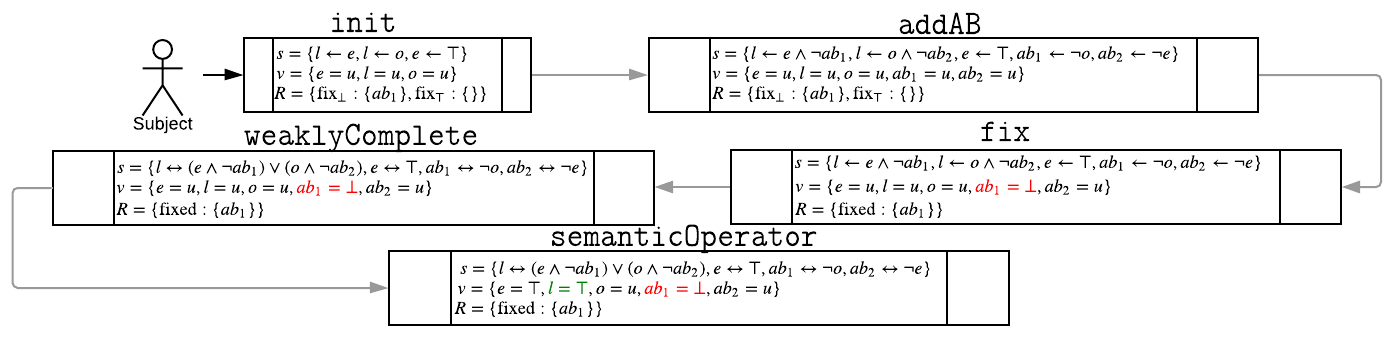
\includegraphics[width=\linewidth]{suppressionSCP_mod2}
\end{center}

\caption{The Suppression Task in which the additional operation of fixing the variable $ab_1$ to false occurs.}
\label{fig:supmod2}
\end{figure*}

The second case of a potential complex operation to add to the search space of our SCPs is the idea of Variable Fixing. The idea that some  conclusions can be fixed \textit{a priori}. Consider a person who strongly doubts the effectiveness of vaccines, we will call her Karen. Karen started her day convinced that giving her child the MMR vaccine is more dangerous than the disease itself. Later that day Karen spoke to her doctor who strongly advised that she vaccinate her child. He offered her a variety of peer-reviewed papers and studies that showed the relative safety of the vaccination. Karen listened carefully to the trained medical professional, and then went home. After some thought Karen decided that he was wrong, and her opinion on vaccines didn't change.

In this example Karen shows a very powerful type of cognitive bias, the unwillingness to change her opinions, despite powerful evidence to the contrary. This phenomenon has been observed across a great many fields of study, from medical psychology \citep{brown2010omission} \citep{wroe2005feeling} to political sciences\citep{tappin2017heart}. In the context of cognitive modelling with logics, it indicates that some mental rules or variables are immutable, regardless of new evidence or valid beliefs that would logically contradict them. Non-monotonic logics, as a class, are already capable of dealing with bias effects, as non-monotonic logics are built on the basis of a preference operation.

 As one possible implementation of this idea, let us introduce a cognitive operation called \texttt{fix}. Fix takes as input any state point and is applicable for any ground point $\bar{p}$ with variable list $V \in \bar{p}$ and categorization variable $R$ with ($fix_\top \lor fix_\bot) \in R$. For all variables $v$ such that $(v \in V) \cap (v \in fix_\top)$ set the value of $v$ to $\top$, For all variables $v$ $(v \in V) \cap (v \in fix_\bot)$ set the value of $v$ to $\bot$. Then remove $fix_\top$ and $fix_\bot$ from $R$. Append $fixed:V_{fix}$ to $R$, where $V_{fix}$ is the set of all variables fixed in this way.

Now, because \texttt{semanticOperator} does not change the values of variables mentioned in $V_{fix} \in fixed:V_{fix}$, $fixed \in R$, Figure~\ref{fig:supmod2} shows the effect of adding a complex operation which fixes the value of the abnormality to false in $v$ so that, no matter what rules in $KB$ when the semantic operator is applied, $ab_1$ will remain false.
\section{Wason Selection Task}

\chapter{Comparing SCPs}
\section{Why do we need to compare SCPs?} \label{sec:whyCompare}
The ability to compare the feasibility of different solutions is an essential step in any computational process in which multiple solutions produce the desired output. Consider a toy example of an SCP task which describes the mental process needed to bake a cake:

\[
\Pi = (s_0, M, \gamma, f())
\]

\[
s_0 = (V=(cakeBaked: \bot) )
\]
\[
M=\{\texttt{mixIngredients}, \texttt{bakeIngredients}, \texttt{doTheLaundry}\}
\]

\[
f(x)= \left\{ \begin{split} cakeBaked \models \top & & & \textrm{True}\\ cakeBaked \models \bot & & & \textrm{False} \end{split} \right\}
\]

\[
\gamma = (f(\pi) = True)
\]

Without specifying the precise details of the complex operations in $M$, and simply using our intuition of the effects of these actions, we can draw some candidate SCPs. Candidate SCPs such as $f(s_0 \longmapsto \texttt{mixIngredients})$ do not result in the cake being baked and so are discounted immediately. However, consider a case where the modelling algorithm being used has come up with two possible SCPs to explain the processes chosen by the participant:

\begin{equation} \label{eq:bakeCake}
SCP_1 = f(s_0\longmapsto \texttt{mixIngredients} \longmapsto \texttt{bakeIngredients})
\end{equation}

\begin{equation} \label{eq:bakeCakeLaundry}
SCP_2 = f(s_0 \longmapsto \texttt{mixIngredients} \longmapsto  \texttt{doTheLaundry} \longmapsto \texttt{bakeIngredients})
\end{equation}

Intuitively, both of these operational sequences would result in a cake being baked and $f(X)$ returning $true$, and thus, both are candidate solutions to the SCP task given. However, both of these solutions may not be equally \textit{plausible}. Why would someone need to do their laundry to make a cake? We can concoct wild scenarios in which the participant's house is so full of dirty laundry that access to the oven it restricted, but this seems implausible. Most readers would agree that Equation~\ref{eq:bakeCake} is more plausible that Equation~\ref{eq:bakeCakeLaundry}.

This toy example is evidence that, in at least some cases, one can confidently prefer one SCP to another. The question now arises: how do we precisely, and consistently prefer one SCP over another? This question is not easy to answer, and this chapter is devoted to proposing candidate solutions which may be able to quantitatively score and select preferable SCPs.

Section~\ref{ssec:compGen} discusses the question of how to compare different SCPs found using search for a single task. Section~\ref{ssec:compExt} discuses the more general problem of comparing SCPs even when the underlying SCPs tasks differ. Section~\ref{ssec:nw} introduces the Needleman-Wunsch Algorithm for string matching whose underlying principles have allowed us to quantify questions of homology and evolutionary relationships in biology, and Section~\ref{ssec:nw_mod} discusses and justifies and extension to this algorithm for use in SCP comparisons.

\section{Comparing Generated SCPs} \label{ssec:compGen}
\subsection{Scoring}
Cognitive modelling as a science that exists, in part, to replicate the empirical results of human reasoning suffers from a painful truth: just because a solution is simple, elegant and seemingly well-justified, it does not follow that that solution is correct. Indeed, that solution might completely fail to explain experimental data from a cognitive task, and must then be discounted. However in the fields of string-matching, etymology, and homological evolution @TODOref3times, mathematically consistent approaches to scoring are still generally a good starting point. And so we carry that assumption into the field of cognitive modellings and assume that, in the absence of directly contradictory empirical data, certain properties related to finding the optimal sequence of cognitive operations are desirable, whilst others are not.

In general the easiest way to compare two distinct objects is to quantify some subset of their properties and use these properties to rank the objects. Continuing with the toy example in Section~\ref{sec:whyCompare} we will attempt to create a commonsense scoring mechanism to determine whether $SCP_1$ or $SCP_2$ is a more cognitively plausible solution to baking a cake. A great many possible criteria exist for scoring these two SCPs, but we will focus on just two of them: the length of the SCP, and the plausibility of each cognitive operation that occurs in either SCP.

\subsubsection{SCP Length}
Perhaps the simplest and most intuitive way to decide which of two SCPs is best suited to solving a specific problem is to prefer the shortest one. In the field of Bioinformatics, one of the earliest approaches to determine which two organisms from a set were more closely related was to directly estimate how many genetic mutations (insertions, deletions, value changes) would be necessary to turn each of these genetic sequences into each other sequence @TODOref. The same logic can be applied to SCPs for those SCPs generated using either \textit{De Novo} or \textit{Insertion Search} (Section~@TODOref).

In the case of \textit{De Novo} search, we assume assume that the optimal length of a solution to $\Pi$ is an SCP length $l=|X|=0$. This optimal solution obviously does not exist in this case $f(s_0) \not\models (cakeBaked = \top)$, but it serves as a way of implicitly preferring shorter SCPs, as those will require fewer insertion operations to satisfy $f(x)$. 

Using this simple test criteria: $|SCP_1| < |SCP_2|$, therefore $SCP_1$ is prefered because it requires only $2$ operations to transform the ideal SCP $f(s_0)$ into $f(s_0\longmapsto \texttt{mixIngredients} \longmapsto \texttt{bakeIngredients})$, rather than the $3$ required for $SCP_2$.

The case for \textit{Insertion search} follows identical logic in order to model deviations from the general reasoner, but uses an ideal SCP which is the known SCP for the general case.

Though simple, this scoring procedure provides the foundations upon which more complex scoring algorithms will be built for the remainder of this section.

\section{Comparing External SCPs} \label{ssec:compExt}
\subsection{The Needleman-Wunsch Algorithm} \label{ssec:nw}
In the field of Bioinformatics, one of the earliest approaches to determine which two organisms from a set were more closely related was to directly estimate how many genetic mutations (insertions, deletions) would be necessary to turn each of these sequences into each other sequence.

\subsection{A Modified Scoring Algorithm} \label{ssec:nw_mod}


\chapter{Program Design}
\section{Implementing the SCP Framework}
The SCP framework has been implemented in \texttt{Python 3} as series of modules which follow strong object-oriented programming principles which support simple extensions and revisions. This implementation is used to demonstrate the practical approaches to generating and evaluating SCPs; and to model a series of cognitive tasks for which empirical results already exist. The library containing this implementation and its associated documentation is available at @TODOref.

At present, concrete implementations for epistemic state structures and cognitive operation formulations related to propositional logic, the WCS, and Reiter's default logic are provided.

\section{A Modular Programming Approach}
% talk about each 
The principle of modular programming is followed in this implementation to the greatest extent possible, thus maximising the ease of modification and upkeep for the program. Figure~@TODOref provides a simplified class diagram to explain how the major components of the system relate to one another.

\subsection{Most Important Modules}

\subsection{Program Flow}
Diagram~@TODOref demonstrates the basic programatic flow used to model the Suppression Task using a WCS SCP. Diagram~@TODOref demonstrates the programmatic flow used by the De Novo search in order to generate an SCP to map to known data. Finally, Diagram~@TODOref shows the process by which information stored in a .csv file can be read into CCOBRA before being interpreted by the SCP framework and used for modelling.

\section{External Framework Integration}


\chapter{Non-Sequential Cognitive Processes}
% relation to neural networks
% summarising tool



\chapter{Conclusions and Future Work}
\section{Conclusion}
SCPs represent a novel and powerful framework for modelling non-monotonic logics. They have been shown capable of modelling the Suppression Task under the WCS for both general and individual cases. SCPs provide a dynamic framework incorporating cognitive operations which are applicable across different logics, provided that those logics share structural features in the initial epistemic state that are compatible with some subset of the known set of cognitive operations. Because the input and output epistemic states need not be structurally similar, SCPs may represent the first approach to modelling human cognition that is able to integrate multiple non-monotonic logic frameworks at run-time and at search-time. 

SCPs represent a new frontier for Cognitive Modelling in non-monotonic logics and research into their capabilities and limitations may help create more robust and mathematically consistent explanations and predictions for human behaviour across an extensive array of cognitive tasks.
\section{Future Work}
The addition of two distinct search paradigms to SCPs may one day enable researchers to generate or test hundreds of thousands of models where only the initial epistemic state is known. The first search type, \textit{De Novo Search}, involves finding an SCP that satisfies a goal condition from scratch, iterating over the set of cognitive operations in $M$. This search is important for producing a computationally valid explanation for the general (most common) results of a cognitive task. \textit{Insertion Search}, by contrast, will require finding which additional complex operations can be added to an existing SCP to produce results consistent with the deviant reasoner. This search is important for describing unusual results as deviations from the general reasoner. It is also important for scoring the likelihood of these with respect to the original SCP. Finally, some form of scoring criteria is needed to compare SCPs to one another and evaluate their relative plausibility with respect to the known complexity of the cognitive operations involved. A modified version of Needleman-Wunsch algorithm for string matching has already been theoretically described and must now be implemented in order to determine how similar different models are to each other.
\chapter*{Appendix}
@TODO talk about adding abnormalities

%----------------------------------------------------------------------------------------
%	THESIS CONTENT - APPENDICES
%----------------------------------------------------------------------------------------

\appendix % Cue to tell LaTeX that the following "chapters" are Appendices

% Include the appendices of the thesis as separate files from the Appendices folder
% Uncomment the lines as you write the Appendices

% Appendix A

\chapter{Frequently Asked Questions} % Main appendix title

\label{AppendixA} % For referencing this appendix elsewhere, use \ref{AppendixA}

\section{How do I change the colors of links?}

The color of links can be changed to your liking using:

{\small\verb!\hypersetup{urlcolor=red}!}, or

{\small\verb!\hypersetup{citecolor=green}!}, or

{\small\verb!\hypersetup{allcolor=blue}!}.

\noindent If you want to completely hide the links, you can use:

{\small\verb!\hypersetup{allcolors=.}!}, or even better: 

{\small\verb!\hypersetup{hidelinks}!}.

\noindent If you want to have obvious links in the PDF but not the printed text, use:

{\small\verb!\hypersetup{colorlinks=false}!}.

%\include{Appendices/AppendixB}
%\include{Appendices/AppendixC}

%----------------------------------------------------------------------------------------
%	BIBLIOGRAPHY
%----------------------------------------------------------------------------------------

\printbibliography[heading=bibintoc]

%----------------------------------------------------------------------------------------

\end{document}  
